\documentclass[11pt]{article}
\renewcommand{\baselinestretch}{1.5}
\setlength{\oddsidemargin}{0pt}
\setlength{\evensidemargin}{0pt}
\setlength{\topmargin}{-20pt}
\setlength{\headsep}{10pt}
\setlength{\headheight}{14pt}
\addtolength{\textheight}{1.3in}
\setlength{\textwidth}{6.2in}
\usepackage{amsmath}
\usepackage{bm}
\usepackage{amsfonts}
\usepackage{enumerate}
\usepackage{tabularx}
\usepackage{makecell}
\usepackage{graphicx}
\usepackage{authblk}
\usepackage{natbib}
\usepackage{caption}
\usepackage{subcaption}
\usepackage{algorithm}
\usepackage{float}
\usepackage{listings}
\usepackage{dsfont}
\usepackage{booktabs}
% \usepackage{algorithmic}
\usepackage{algpseudocode} % for the algorithmic environment
\usepackage{multirow}
\usepackage{booktabs}
\usepackage[colorlinks=true, linkcolor=blue, urlcolor=blue]{hyperref}





\newtheorem{lemma}{Lemma}


\title{Animal Trajectory Imputation and Uncertainty Quantification Using Deep Learning}

\author[1]{Kehui Yao}

\affil[1]{Department of Statistics, University of Wisconsin-Madison}




\date{}

\begin{document}

\maketitle

\begin{abstract}
Imputing missing data in animal trajectories is crucial for understanding their movements during unobserved periods. Traditional methods such as linear interpolation and the continuous-time correlated random walk model often fail to capture the complexity of animal movements, making the imputation less accurate. Here we develop a deep learning approach to animal trajectory imputation, using the Conditional Score-based Diffusion Model (CSDI) originally designed for multivariate time series data. Unlike traditional methods, our deep learning method uses observed trajectories and external covariates to impute missing locations, capturing periodic patterns and the influence of covariates on animal movements, which leads to more accurate imputations. We develop a pipeline to segment trajectories from hundreds of deer and train the model to learn general movement patterns from this collective dataset. When tested on a dataset of 402 female deer trajectories in Wisconsin, our method not only achieves more accurate deterministic imputations but also more reliable probabilistic imputations than existing methods.

\end{abstract}

\textbf{keywords}: Animal Trajectory Imputation, Deep Learning, Conditional Scored-based Diffusion Model
\section{Introduction}
Animal movement data often includes spatial positions recorded at specific time points using GPS telemetry technology. Although these locations are usually sampled at regular intervals, data gaps are inevitable due to collection issues or noise. A variety of statistical and machine learning methods have been used in an effort to fill in such missing data.

One common method, linear interpolation, estimates missing values by drawing straight lines between observed data points. Essentially, it assumes a linear relationship between consecutive points and interpolates the missing values accordingly.
 However, this method has several drawbacks. First, the estimation is too simple, failing to capture the complex dynamics of animal movement. Secondly, the imputation is deterministic, which means it fails to account for the inherent uncertainty in predicting the path between observed locations.
 Beyond linear interpolation, several statistical methods are used to analyze animal movement data. Hidden Markov Models (HMMs) 
and State-Space Models (SSMs) are effective in analyzing datasets with consistent time intervals
\citep{holzmann2006hidden, patterson2009classifying, mckellar2015using, towner2016sex, breed2012state}. 
 Continuous time models are more suitable for datasets with irregular or continuous time intervals
\citep{johnson2008continuous, buderman2016functional}. These methods are parametric. Once fitted to the observed data, predict the missing locations of animals at specified time points. Additionally, these models naturally incorporate uncertainty. However, these statistical models have limitations. First, these methods often require expert knowledge of animal movement patterns and ecological insights because accurate model specification is crucial. They often lack the flexibility to identify patterns or to understand complex, nonlinear environmental interactions directly from the observed data. Second, those methods typically model the movement of only one animal at a time and do not share information across individuals. Previously, this was reasonable due to limited data availability. However, modern GPS technology now enables the simultaneous tracking of multiple animals, providing the opportunity to leverage collective data for enhanced imputation.

Machine learning and deep learning methods often provide superior pattern extraction capabilities compared to traditional statistical methods. Researchers have explored these methods for animal trajectory analysis. Examples include the RandomForest approach by \citet{rew2019animal}, inverse reinforcement learning by \citet{hirakawa2018can}, and the LSTM encoder-decoder network by \citet{li2021prediction}. Despite their potential, deep learning's adoption for animal trajectory imputation remains limited. This limited adoption may be due to several factors. A major concern is that most deep learning models produce deterministic predictions, while a probabilistic approach providing a range of possible locations might better predict an animal's potential positions. Furthermore, deep learning requires extensive training data. In situations with limited data, such as tracking a few animals, these models may learn more noise than underlying patterns. Lastly, methods like LSTM and RandomForest, designed primarily for datasets with regular time intervals, are not suitable for those with irregular intervals.


In our study, we extend the Conditional Score-based Diffusion Models (CSDI) \citep{tashiro2021csdi}, originally designed for probabilistic time series imputation, to the context of animal trajectory imputation. Figure \ref{fig: visualization of the CSDI for trajectory imputation} shows the procedure of this algorithm. We prepare a large training dataset by segmenting the trajectories of 402 deer. The proposed model imputes missing trajectories based on observed locations and by incorporating the deer's habitat landcover and temporal information. Our study shows that the model significantly outperforms traditional trajectory imputation methods, such as linear interpolation and the continuous-time correlated random walk model \citep{johnson2008continuous} in both mean absolute error (MAE) and continuous ranked probability score (CRPS) metrics. Additionally, this model addresses the two main challenges previously outlined: it can impute data with irregular time intervals and produce uncertainty quantifications via probabilistic imputations. To our knowledge, this is the first work to apply generative models to animal trajectory imputation with uncertainty quantification.
 
 
\begin{figure}[h]
  \centering
  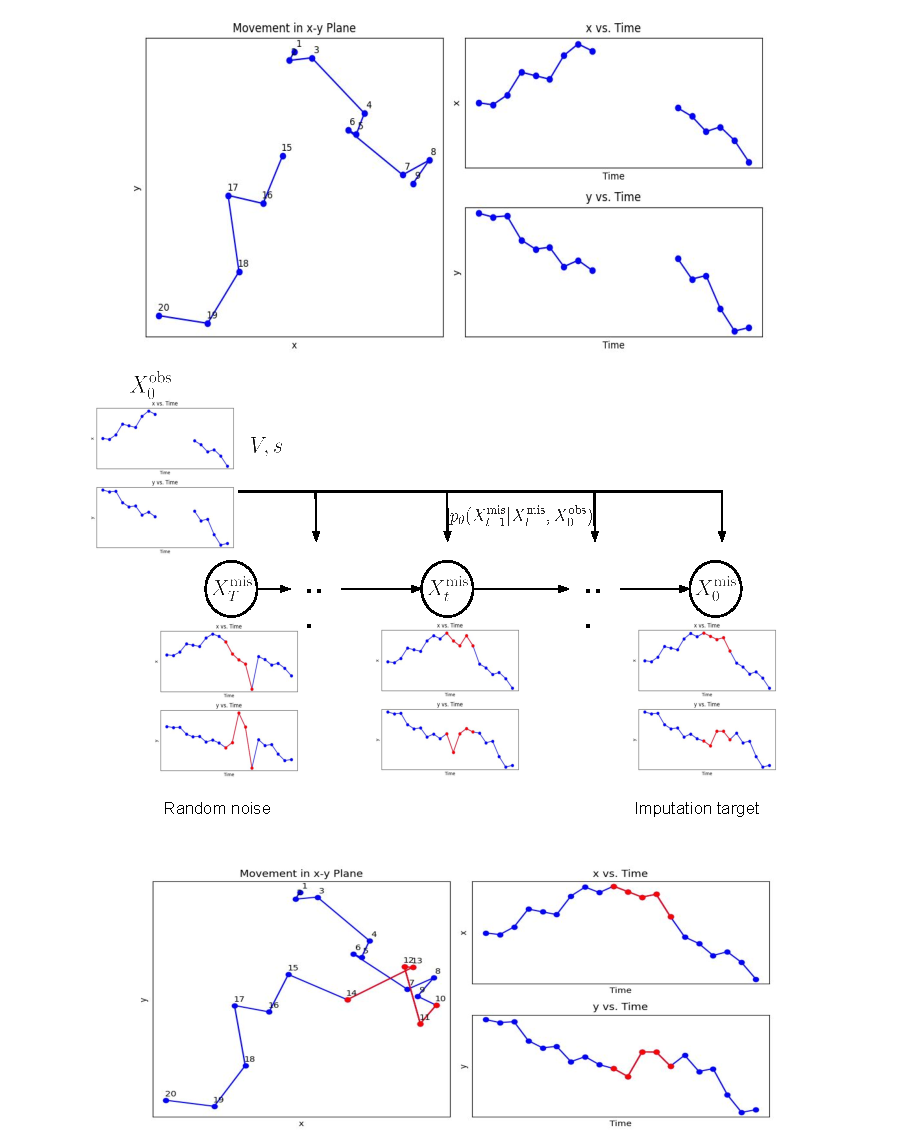
\includegraphics[width=\textwidth]{../figure/algorithm} % Adjust the scale or width as needed
  \caption{Procedure for the CSDI algorithm for trajectory imputation. First, the trajectory is decomposed into a bivariate time series with missing values. Then this bivariate time series is input into the CSDI model to impute the missing values. Finally, the imputed values are then reassembled back into the original trajectory. In the figure, black ``x" marks represent observed data points, while unfilled black ``o" circles indicate imputed data points.}
  \label{fig: visualization of the CSDI for trajectory imputation} % Label for referencing
\end{figure}



%Denote $\mathcal{X}$ as the sample space for $\bm{X}$, $\bm{X}^{\mathrm{obs}}$, and $\bm{X}^{\mathrm{mis}}$.


%\section{Traditional Method}

%In this section, we explore two traditional methods commonly used for animal trajectory imputation: linear interpolation and the continuous-time correlated random walk (CTCRW) model \citep{johnson2008continuous}.
%
%\subsection{Linear Interpolation}
%Linear interpolation, a straightforward method, involves drawing a straight line between two known points to estimate missing values for any intervening points. This method is advantageous due to its simplicity and minimal computational demands. However, this imputation may lack accuracy because it overlooks the animal's movement patterns and external environmental factors.

%\section{Continuous-Time Correlated Random Walk Model}
%\citet{johnson2008continuous} introduced the continuous-time correlated random walk (CTCRW) model, specifically designed to analyze animal telemetry data collected at irregular time intervals. At its core, the model uses the continuous-time Ornstein-Uhlenbeck process to model the animal's movement velocity. To estimate movement parameters and predict unobserved locations, the model uses a state-space framework. Detailed procedures for applying the CTCRW model to impute missing trajectory data are shown in Section \ref{sec: imputation using ctcrw}.
%\subsection{RandomForest}
%Random Forest is a machine learning method well-suited for imputing missing values in time series data. It works by constructing numerous decision trees, each based on different subsets of the data and features, to make predictions. For time series imputation, Random Forest takes into account the sequential nature of the data and any relevant external variables, utilizing the relationships between time points to predict missing values accurately. The details of implementing RandomForest for animal trajectory imputation can be seen in Appendix \ref{sec: randomforest}.

\section{Model}
\subsection{Notations for Animal Trajectory Data}\label{sec: multivariate time series imputation}
Consider a collection of $N$ trajectories with missing data, each associated with either a single animal or a group of animals. Telemetry data is represented as $\bm{X} \in \mathbb{R}^{2 \times L}$, where ``2" denotes the two spatial coordinates (longitude and latitude), and $L$ represents the trajectory's length. To distinguish between missing and observed data, we use an observation mask $\bm{M} \in \{0,1\}^{2 \times L}$. Here, $\bm{M}[c,l]=0$ indicates that $\bm{X}[c,l]$ is missing, and $\bm{M}[c,l]=1$ indicates that $\bm{X}[c,l]$ is observed, for $c\in \{1,2\}$ and $l \in \{1,\ldots,L\}$. It is important to note that the time intervals between consecutive data points may vary, denoted by $\bm{s} \in \mathbb{R}^L$. Additionally, we include relevant information for each trajectory in $\bm{V} \in \mathbb{R}^{L \times K}$, where $K$ is the dimension of information. In summary, each trajectory is represented by the set $\{\bm{X}, \bm{M}, \bm{V}, \bm{s}\}$. We define $\bm{X}^{\mathrm{obs}} = \bm{X} \odot \bm{M}$ as the observed and $\bm{X}^{\mathrm{mis}} = \bm{X} \odot (\bm{1}-\bm{M})$ as the missing that requires imputation. 

%Figure \ref{fig: visualization of the CSDI for trajectory imputation} shows the procedure of this algorithm.

\subsection{Denoising Diffusion Probabilistic Models}\label{sec: ddpm}
Assume we want to estimate a true data distribution $q(\bm{X}_0)$. The objective of DDPM is to train a model $p_{\theta}(\bm{X}_0)$, to closely match the true data distribution $q(\bm{X}_0)$ by working with a sequence of latent variables $\bm{X}_t$, (for $t=1$ to $T$), which exist in the same sample space as $\bm{X}_0$. Following the diffusion probabilistic model framework introduced by \citet{ho2020denoising}, the approach consists of two main stages: a forward process and a reverse process.
\subsubsection*{Forward Diffusion Process}
The forward process begins by sampling a data point $\bm{X}_0$ from an actual data distribution $q(\bm{X}_0)$, and then incrementally introduces Gaussian noise over $T$ steps, yielding a series of increasingly noisy samples $\bm{X}_1,\ldots,\bm{X}_T$. The step sizes are controlled by a predetermined sequence of variances, $\{\beta_t\in(0,1)\}_{t=1}^T$. The forward diffusion process can be expressed as:


\begin{align}\label{eq: forward diffusion}
	&q(\bm{X}_{1:T}|\bm{X}_0)=\prod_{t=1}^{T}q(\bm{X}_t|\bm{X}_{t-1})\\
	&q(\bm{X}_t|\bm{X}_{t-1})=\mathcal{N}(\sqrt{1-\beta_t}\bm{X}_{t-1}, \beta_t\bm{\mathrm{I}}).
\end{align}
Based on the forward process, we can sample $\bm{X}_t$ at any arbitrary time step $t$ directly from the initial data point $\bm{X}_0$, using the distribution $q(\bm{X}_t|\bm{X}_0)=\mathcal{N}(\bm{X}_t;\sqrt{\alpha_t}\bm{X}_0, (1-\alpha_t)\bm{\mathrm{I}})$, where $\alpha_t=\prod_{i=1}^t (1-\beta_i)$.  Therefore, $\bm{X}_t=\sqrt{\alpha_t}\bm{X}_0+(1-\alpha_t)\bm{\epsilon}$, where $\bm{\epsilon}\sim \mathcal{N}(0, \bm{\mathrm{I}})$. 


\subsubsection*{Reverse Diffusion Process}

The objective of reversing the diffusion process is to reconstruct the original data point starting from Gaussian noise, denoted as $\bm{X}_T \sim \mathcal{N}(\bm{0}, \bm{\mathrm{I}})$. However, directly calculating the reverse conditional probabilities $q(\bm{X}_{t-1}|\bm{X}_t)$ is challenging. As a solution, a model $p_{\theta}$ is trained to approximate these conditional probabilities and to execute the reverse diffusion. The reverse diffusion process can be expressed as:
\begin{align}\label{eq: reverse diffusion}
	&p_{\theta}(\bm{X}_{0:T})=p(\bm{X}_T)\prod_{t=1}^Tp_{\theta}(\bm{X}_{t-1}|\bm{X}_t)\\
	&p(\bm{X}_T)\sim \mathcal{N}(\bm{0}, \bm{\mathrm{I}})\\
	&p_{\theta}(\bm{X}_{t-1}|\bm{X}_t)=\mathcal{N}(\bm{X}_{t-1};\bm{\mu}_{\theta}(\bm{X}_t, t), \sigma_{\theta}(\bm{X}_t, t)\bm{\mathrm{I}})
\end{align}
\citep{ho2020denoising} considers the following parameterization of $\bm{\mu}_{\theta}(\bm{X}_t, t)$ and $\sigma_{\theta}(\bm{X}_t, t)$:
\begin{align}\label{eq: DDPM parametrization}
	&\bm{\mu}_{\theta}(\bm{X}_t, t)=\frac{1}{\alpha_t}\{\bm{X}_t-\frac{\beta_t}{\sqrt{1-\alpha_t}}\bm{\epsilon}_{\theta}(\bm{X}_t, t)\}\\
	&\sigma_{\theta}(\bm{X}_t, t)=\tilde{\beta}_t^{1/2}\\
	&\tilde{\beta}_t= \begin{cases}\frac{1-\alpha_{t-1}}{1-\alpha_t} \beta_t & t>1 \\ \beta_1 & t=1\end{cases}
\end{align}
where $\bm{\epsilon}_{\theta}$ is a trainable denoising function. We denote $\bm{\mu}_{\theta}(\bm{X}_t,t)$ and $\sigma_{\theta}(\bm{X}_t, t)$ in Eq. \ref{eq: DDPM parametrization} as $\bm{\mu}^{\mathrm{DDPM}}(\bm{X}_t, t, \bm{\epsilon}_{\theta}(\bm{X}_t, t))$ and $\sigma^{\mathrm{DDPM}}(\bm{X}_t, t)$, respectively. Under this parameterization, \citet{ho2020denoising} have shown that the reverse process can be trained by solving the following optimization problem:
\begin{align}
	&\min_{\theta}\mathcal{L}(\theta)=\min_{\theta}\mathbb{E}_{t\sim [1,T],\bm{X}_0,\bm{\epsilon}}||\bm{\epsilon}-\bm{\epsilon}_{\theta}(\bm{X}_t, t)||^2_2\\
	&\mbox{where } \bm{X}_t=\sqrt{\alpha_t}\bm{X}_0+(1-\alpha_t)\bm{\epsilon}.
\end{align}
This optimization function implies that the denoising function $\bm{\epsilon}_{\theta}$ estimates the noise vector $\bm{\epsilon}$ that was added to its noisy input $\bm{X}_t$. Once trained, we can sample $\bm{X}_0$ from Eq. \ref{eq: reverse diffusion}. More details of DDPM can be found in Appendix \ref{sec: DDPM details}.



\section{Method}
\subsection{Imputation with Conditional Diffusion Models}\label{sec: csdi}
Let's assume the missing data $\bm{X}^{\mathrm{mis}}$ follows a distribution $q(\bm{X}^{\mathrm{mis}}|\bm{X}^{\mathrm{obs}}, \bm{V}, \bm{s})$, which is conditioned on the observed data $\bm{X}^{\mathrm{obs}}$ and additional variables $\bm{V}$ and $\bm{s}$. Our goal is to construct a model denoted by $p_{\theta}(\bm{X}^{\mathrm{mis}}|\bm{X}^{\mathrm{obs}}, \bm{V}, \bm{s})$ that can closely approximate this true distribution $q$. Consider modeling $p_{\theta}(\bm{X}_0^{\mathrm{mis}}|\bm{X}_0^{\mathrm{obs}}, \bm{V}, \bm{s})$ with a diffusion model by extending the reverse process in Eq. \ref{eq: reverse diffusion} to a conditional format:
\begin{align}\label{eq: conditional reverse process}
	&p_{\theta}(\bm{X}_{0:T}^{\mathrm{mis}}|\bm{X}_0^{\mathrm{obs}}, \bm{V}, \bm{s})=p(\bm{X}_T^{\mathrm{mis}})\prod_{t=1}^T p_{\theta}(\bm{X}_{t-1}^{\mathrm{mis}}|\bm{X}_t^{\mathrm{mis}},\bm{X}_0^{\mathrm{obs}},\bm{V},\bm{s})\\
	&\bm{X}_T^{\mathrm{mis}}\sim \mathcal{N}(\bm{0},\bm{\mathrm{I}})\\
	&p_{\theta}(\bm{X}_{t-1}^{\mathrm{mis}}|\bm{X}_t^{\mathrm{mis}},\bm{X}_0^{\mathrm{obs}})=\mathcal{N}\{\bm{X}_{t-1}^{\mathrm{mis}};\bm{\mu}_{\theta}(\bm{X}_t^{\mathrm{mis}}, t|\bm{X}_0^{\mathrm{obs}},\bm{V},\bm{s}), \sigma_{\theta}(\bm{X}_t^{\mathrm{mis}},t|\bm{X}_0^{\mathrm{obs}},\bm{V},\bm{s})\bm{\mathrm{I}}\}
\end{align}
Based on Eq. \ref{eq: conditional reverse process}, we aim to model the conditional distribution $p_{\theta}(\bm{X}_{t-1}^{\mathrm{mis}}|\bm{X}_t^{\mathrm{mis}},\bm{X}_0^{\mathrm{obs}},\bm{V}, \bm{s})$. Specifically, we extend the unconditional DDPM in Eq. \ref{eq: DDPM parametrization} to the following conditional case. 
\begin{align}\label{eq: conditional DDPM parametrization}
	&\bm{\mu}_{\theta}(\bm{X}_t^{\mathrm{mis}}, t|\bm{X}_0^{\mathrm{obs}},\bm{V},\bm{s})=\bm{\mu}^{\mathrm{DDPM}}(\bm{X}_t^{\mathrm{mis}},t,\bm{\epsilon}_{\theta}(\bm{X}_t^{\mathrm{mis}},t|\bm{X}_0^{\mathrm{obs}},\bm{V},\bm{s}))\\
	&\sigma_{\theta}(\bm{X}_t^{\mathrm{mis}},t|\bm{X}_0^{\mathrm{obs}},\bm{V},\bm{s})=\sigma^{\mathrm{DDPM}}(\bm{X}_t^{\mathrm{mis}},t)
\end{align}
where $\bm{\epsilon}_{\theta}$ becomes the conditional denoising function that takes conditional observations $\bm{X}_0^{\mathrm{obs}}$ and auxiliary information $\bm{V}$ and $\bm{s}$ as inputs. $\bm{\mu}^{\mathrm{DDPM}}$ and $\sigma^{\mathrm{DDPM}}$ in Eq. \ref{eq: conditional DDPM parametrization} are the same functions defined in Eq. \ref{eq: DDPM parametrization}. 
 

Once trained, given the function $\bm{\epsilon}_{\theta}$, $\bm{X}_0^{\mathrm{obs}}$, $\bm{V}$, and $\bm{s}$, we can sample $\bm{X}_0^{\mathrm{mis}}$ based on the reverse process in Eq. \ref{eq: conditional reverse process}. 

\subsection{Training and Imputation}\label{sec: training of csdi}
It is important to note that the form of $\bm{\epsilon}_{\theta}$ is the only difference between the parametrization in Eq. \ref{eq: conditional DDPM parametrization} and Eq. \ref{eq: DDPM parametrization}. Consequently, the training process for the conditional denoising function follows the same procedure as the unconditional model in Section \ref{sec: ddpm}. Given conditional observations $\bm{X}_0^{\mathrm{obs}}$, $\bm{V}$, $\bm{s}$ and imputation targets $\bm{X}_0^{\mathrm{mis}}$, we sample noisy targets $\bm{X}_t^{\mathrm{mis}}=\sqrt{\alpha_t}\bm{X}_0^{\mathrm{mis}}+(1-\alpha_t)\bm{\epsilon}$, and train $\bm{\epsilon}_{\theta}$ by minimizing the following loss function:
\begin{equation}\label{eq: objective function}
	\min_{\theta}\mathcal{L}(\theta)=\min_{\theta}\mathbb{E}_{t\sim [1,T],\bm{X}_0^{\mathrm{mis}},\bm{\epsilon}}||\bm{\epsilon}-\bm{\epsilon}_{\theta}(\bm{X}_t^{\mathrm{mis}}, t|\bm{X}_0^{\mathrm{obs}},\bm{V},\bm{s})||^2_2,
\end{equation}


However, in practical scenarios, the ground-truth values for $\bm{X}_0^{\mathrm{mis}}$ are typically unknown during training. To address this, CSDI uses a self-supervised learning strategy, that is, for a given sample $\bm{X}_0$, the observed part of $\bm{X}_0^{\mathrm{obs}}$ are further separated into two parts, one serving as imputation targets, denoted as $\bm{X}_0^{\mathrm{ta}}$, and the other as conditional observations $\bm{X}_0^{\mathrm{co}}$. 


Once we obtain $\bm{X}_0^{\mathrm{ta}}$ and $\bm{X}_0^{\mathrm{co}}$, we proceed by substituting $\bm{X}_0^{\mathrm{mis}}$ with $\bm{X}_0^{\mathrm{ta}}$, $\bm{X}_0^{\mathrm{obs}}$ with $\bm{X}_0^{\mathrm{co}}$,  and train $\bm{\epsilon}_{\theta}$ in Eq. \ref{eq: objective function}. The details of the training algorithm are shown in Algorithm \ref{alg: training}.



\begin{algorithm}
\caption{Training of CSDI}\label{alg: training}
\begin{algorithmic}[1] % Enables line numbering
\State \textbf{Input:} Training data distribution $q(\cdot)$, masking strategy $\mathcal{T}$, the number of iterations $n_{\mathrm{iter}}$, and the sequence of noise levels $\{\alpha_t\}$.
\State \textbf{Output:} Trained denoising function $\bm{\epsilon}_{\theta}$.
\For{$i=1$ \textbf{to} $n_{\mathrm{iter}}$}
    \State Sample $t$ from Uniform$(\{1,\ldots, T\})$, Sample $\{\bm{X}_0, \bm{M}, \bm{V}, \bm{s}\}$ from $q(\cdot)$.
    \State Apply the strategy $\mathcal{T}$ to separate $\bm{X}_0$ into conditional  observations $\bm{X}_0^{\mathrm{co}}$ and imputation targets $\bm{X}_0^{\mathrm{ta}}$.
    \State Sample $\bm{\epsilon}$ from $\mathcal{N}(\bm{0}, \mathrm{I})$, where $\bm{\epsilon}\in \mathcal{X}$.
    \State Compute noisy targets $\bm{X}_t^{\mathrm{ta}}=\sqrt{\alpha}_t \bm{X}_0^{\mathrm{ta}} + (1-\alpha_t)\bm{\epsilon}$.
    \State Update $\bm{\epsilon}_{\theta}$ by minimizing the squared error loss $\left\|\left(\boldsymbol{\epsilon}-\boldsymbol{\epsilon}_\theta\left(\mathbf{X}_t^{\mathrm{ta}}, t \mid \bm{X}_0^{\mathrm{co}},\bm{V}_j,\bm{s}_j\right)\right)\right\|_2^2$.
\EndFor
\end{algorithmic}
\end{algorithm}


Once the $\bm{\epsilon}_{\theta}$ is trained, we follow Eq. \ref{eq: conditional reverse process} to generate $\bm{X}_0^{\mathrm{mis}}$. The steps involved in the imputation process are outlined in Algorithm \ref{alg: imputation}.

\begin{algorithm}
\caption{Imputation (Sampling) with CSDI}\label{alg: imputation}
\begin{algorithmic}[1] 
\State \textbf{Input}: a data sample $\{\bm{X}_0,\bm{M},\bm{V}, \bm{s}\}$, a trained denoising function $\bm{\epsilon}_{\theta}$.
\State \textbf{Output}: Imputed missing values $\bm{X}_0^{\mathrm{mis}}$.
\State Initialize $\bm{X}_T^{\mathrm{mis}}$ by sampling from  $\mathcal{N}(\bm{0}, \bm{\mathrm{I}})$, where $\bm{X}_T^{\mathrm{mis}}\in \mathcal{X}$.
\For{$t=T$ \textbf{to} $1$}     \State Compute $\bm{X}_{t-1}^{\mathrm{mis}}$ using Eq. \ref{eq: conditional reverse process} and Eq. \ref{eq: conditional DDPM parametrization}.
\EndFor
\State Output the final imputed values
 $\bm{X}_0^{\mathrm{mis}}$.
\end{algorithmic}
\end{algorithm}



\subsection{Architecture of the Denoising Function}
In this section, we briefly describe the architecture of the denoising function $\bm{\epsilon}_{\theta}$. At its core, $\bm{\epsilon}_{\theta}$ is designed as a neural network with multiple residual layers and channels. The complete structure of $\bm{\epsilon}_{\theta}$ is detailed in \citet{tashiro2021csdi}.

The model inputs include the observed data $\bm{X}_0^{\mathrm{obs}}$, the missing data $\bm{X}_t^{\mathrm{mis}}$, covariate $\bm{V}$, time intervals $\bm{s}$, and a diffusion step $t$. The model uses a 128-dimensional embedding for 
the diffusion step $t$ and $\bm{s}$ \citep{vaswani2017attention} and uses a 64-dimensional feature embedding for $\bm{V}$. The temporal embedding for diffusion step $t$ and time interval $\bm{s}$ are expressed as follows:
\begin{equation}
	\mathrm{DiffusionEmbed}(t)=\{\sin(10^{0\cdot 4/63}t),\ldots, \sin(10^{63\cdot 4/63}t), \cos(10^{0\cdot 4/63}t),\ldots,\cos(10^{63\cdot 4/63}t)\}.
\end{equation}
\begin{equation}
	\mathrm{TimeEmbed}(s_l)=\{\sin(s_l/\tau^{0/64}),\ldots, \sin(s_l/\tau^{63/64}), \cos(s_l/\tau^{0/64}),\ldots,\cos(s_l/\tau^{63/64})\},
\end{equation}
where $\tau=10000$. 


Within each residual layer, the model uses a single-layer Transformer Encoder. This encoder includes a multi-head attention layer, fully connected layers, and layer normalization. These components are designed to effectively capture both temporal and feature-based dependencies within multivariate time series data. 







\section{Case Study}
\subsection{Dataset}
Our dataset 402 female deer tracked across Wisconsin. For each deer, locations were recorded at multiple time points. Here, locations are recorded as pairs of geographic coordinates and times are recorded in Julian days, beginning on January 1, 2017. Time points are generally spaced 4 hours apart, with gaps indicating missing data for those intervals. On average, approximately 2700 observations were recorded for each deer. Besides location tracking, the dataset includes information on the landscapes traversed by the deer, categorized by the National Land Cover Database (NLCD) classifications \citep{usgs_nlcd_2011}. Additionally, each observation's timing is detailed down to the month, day, and hour, with the month variable being a critical indicator for various seasonal activities like breeding, fawning, nonbreeding, or post-fawning.
\subsection{Notation}
Let $N$ represent the total number of deer trajectories. For each deer $j$, let $n_j$ be the number of observed time points, $\bm{t}_j = \{t_{j1}, \ldots, t_{jn_j}\}$ the specific observation times, $\bm{Y}_j \in \mathbb{R}^{2 \times n_j}$ the location coordinates, and $\bm{Z}_j \in \mathbb{R}^{n_j \times K}$ the auxiliary information. The auxiliary information includes landscape and time-related variables. The landscape variable is categorized into 15 unique land cover types. Each category is transformed into a 15-dimensional one-hot encoded vector, with each dimension representing a distinct land cover type. Additionally, time-related variables like the month, day, and hour of observation contribute three more dimensions to $\bm{Z}_j$, resulting in a total of 18 dimensions ($K=18$). Here, the complete dataset for deer $j$ is represented by $\{\bm{Y}_j, \bm{Z}_j, \bm{t}_j\}$.


Our ultimate goal is to reconstruct the paths of each deer to ensure their movements are recorded at regular 4-hour intervals. To achieve this, $\bm{t}_j$ is expanded into an augmented series $\bm{t}_j^{\mathrm{aug}}=\{t_{j1}^{\mathrm{aug}},\ldots,t_{jm_j}^{\mathrm{aug}}\}$, with $n_j^{\mathrm{aug}}$ denoting the series length. Define $t_{j1}^{\mathrm{aug}}=t_{j1}$, $t_{jn_j^{\mathrm{aug}}}^{\mathrm{aug}}=t_{jn_j}$, $\bm{t}_j\subseteq \bm{t}_j^{\mathrm{aug}}$, and the interval between $t_{ji}^{\mathrm{aug}}$ and $t_{j,i-1}^{\mathrm{aug}}$ as 4 hours. Additionally, the deer's location data for the augmented time points is denoted by $\bm{Y}_j^{\mathrm{aug}}\in \mathbb{R}^{2\times n_j^{\mathrm{aug}}}$, and the associated auxiliary information by $\bm{Z}_j^{\mathrm{aug}}$. Time points in $\bm{t}_j^{\mathrm{aug}}$ not found in the original $\bm{t}_j$ indicate intervals with missing location data we aim to reconstruct. Define $\bm{P}_j^{\mathrm{aug}}\in \mathbb{R}^{2\times n_j^{\mathrm{aug}}}$ as the mask for identifying missing versus observed data. Therefore, our task is to impute missing values in $\bm{Y}_j^{\mathrm{aug}}$.



Evaluating the effectiveness of various imputation methods for $\bm{Y}_j^{\mathrm{aug}}$ is challenging due to the absence of true missing data values, making direct evaluation infeasible. We address this challenge using a self-supervised learning approach. We first partition our dataset into training and testing subsets. Specifically, we randomly select $80\%$ (331 individuals) to form the training dataset, denoted as $\mathcal{D}_{\mathrm{train}}$. The remaining $20\%$ (71 individuals) form the testing dataset, denoted as $\mathcal{D}_{\mathrm{test}}$. For each deer $j$ in $\mathcal{D}_{\mathrm{test}}$, we randomly select $p\%$ of the time points from $\bm{t}_j$ and mark the corresponding location data $\bm{Y}_j$ and associated covariates $\bm{Z}_j$ as missing. The resulting datasets are defined as $\{\bm{Y}_j^{\mathrm{test}},\bm{Z}_j^{\mathrm{test}}, \bm{t}_j, \bm{P}_j^{\mathrm{test}}\}$, with $\bm{P}_j^{\mathrm{test}}$ as the mask identifying observed versus missing data. We then use various methods to impute $\bm{Y}_j^{\mathrm{test}}$ and evaluate their performance by comparing the imputed data with the true data of $\bm{Y}_j$. Let $\hat{\bm{Y}}_j^{\mathrm{test}}$ denote the deterministic imputation of $\bm{Y}_j^{\mathrm{test}}$. The Mean Absolute Error (MAE) is defined as:
\begin{equation}
	\mathcal{L}=\frac{\sum_{j\in \mathcal{D}_{\mathrm{test}}}\sum \big\{|\hat{\bm{Y}}_j^{\mathrm{test}}-\bm{Y}_j|\odot (\bm{1}-\bm{P}_j^{\mathrm{test}})\big\}}{\sum_{j\in \mathcal{D}_{\mathrm{test}}}\sum (\bm{1}-\bm{P}_j^{\mathrm{test}})}.
\end{equation} 
In probabilistic imputation, treat the imputed test matrix $\bm{Y}_j^{\mathrm{test}}$, denoted by $\tilde{\bm{Y}}_j^{\mathrm{test}}$, as a matrix of random variables following a specific probability distribution $\bm{F}_j^{\mathrm{test}}$. To assess probabilistic imputation accuracy, we use the continuous ranked probability score (CRPS)\citep{matheson1976scoring}. CRPS calculates the integral of the quantile loss, $\Lambda_\alpha(q, z) = (\alpha - \mathbb{I}_{z < q})(z - q)$, for a scalar $y$ and its estimated probability distribution $F$, across all quantile levels $\alpha$ in the interval $[0,1]$: \begin{equation}
    \operatorname{CRPS}\left(F, y\right)=\int_0^1 2 \Lambda_\alpha\left(F^{-1}(\alpha), y\right) \mathrm{d} \alpha
\end{equation}
If $F$ is not tractable, we generate 100 samples to approximate it for each missing value, following \citet{tashiro2021csdi}. We calculate quantile losses at discrete quantile levels, using increments of 0.05: \begin{equation}
    \operatorname{CRPS}\left(F, y\right) \simeq \sum_{i=1}^{19} 2 \Lambda_{i * 0.05}\left(F^{-1}(i * 0.05), y\right) / 19
\end{equation}
If $\bm{Y}$ is a matrix of random variables with $\bm{F}$ as its elementwise probability distribution, where $F_{ij}$ is the distribution for $y_{ij}$, the CRPS calculation is: \begin{equation}
    \operatorname{CRPS}\left(\bm{F}, \bm{y}\right) = \frac{\sum_{i,j}\mathrm{CRPS}(F^{-1}_{i,j},y_{i,j})}{\sum_{i,j}|y_{i,j}|}
\end{equation}
Therefore, the CRPS for our testing dataset is calculated as: \begin{equation}
    \mathcal{L}=\frac{\sum_{j\in \mathcal{D}_{\mathrm{test}}}\sum \big\{\mathrm{CRPS}(\bm{F}^{\mathrm{test}}_j,\bm{Y}_j)\odot (\bm{1}-\bm{P}_j^{\mathrm{test}})\big\}}{\sum_{j\in \mathcal{D}_{\mathrm{test}}}\sum\{\bm{Y}_j^{\mathrm{test}}\odot (\bm{1}-\bm{P}_j^{\mathrm{test}})\}},
\end{equation}



\subsection{Imputation Using Existing Method}\label{sec: imputation using ctcrw}

\citet{johnson2008continuous} introduced the continuous-time correlated random walk (CTCRW) model, specifically designed to analyze animal telemetry data collected at irregular time intervals. At its core, the model uses the continuous-time Ornstein-Uhlenbeck process to model the animal's movement velocity. To estimate movement parameters and predict unobserved locations, the model uses a state-space framework. 

We define each animal's bivariate location data at time $t$ as $\bm{\mu}(t)=[\mu_1(t), \mu_2(t)]^{\prime}$. Define $d\bm{\mu}(t)=\bm{v}(t)dt$, where $\bm{v}(t)$ is the instantaneous rate of location change (velocity). For each coordinate axis ($c=1, 2$), we define the Ornstien-Uhlenbeck (OU) process $v_c(t)$ as follows:
\begin{equation}\label{eq: velocity}
    v_c(t+\Delta)=\gamma_c+e^{-\beta\Delta}[v_c(t)-\gamma_c]+\zeta_c(\Delta),
\end{equation}
where $\gamma_c$ is the mean velocity, $\beta$ is an autocorrelation parameter, and $\zeta_c(\Delta)$ is a zero mean normal random variable with variance $\sigma^2[1-\exp(-2\beta\Delta)]/2\beta$. The parameter $\sigma$ controls the overall variability in velocity.

Using the velocity process, we obtain the continuous-time location process $\bm{\mu}(t)$ by integration as shown:
\begin{equation}\label{eq: location}
    \bm{\mu}(t)=\bm{\mu}(0)+\int_{0}^{t}\bm{v}(u)du.
\end{equation}
Equations \ref{eq: velocity} and \ref{eq: location} define the basic continuous-time correlated random walk model (CTCRW).

However, the continuous path of an animal can only be observed at sampled times. Assume locations $\bm{y}_i = [y_{1i}, y_{2i}]$ are measured at times $t_1, \ldots, t_n$, and that the true locations $\bm{\mu}_i = [\mu_{1i}, \mu_{2i}]'$ of the animal at each time $t_i$ allow us to represent CTCRW within a state-space model framework. 

\begin{align}\label{eq: general ssm}
	&y_{ci}=Z_i^{\prime}\bm{\alpha}_{ci}+\epsilon_{ci}\\
	&\bm{\alpha}_{c,i+1}=T_i\bm{\alpha}_{ci}+\bm{\eta}_{ci},
\end{align}
where $Z_i=[1, 0]^{\prime}$, $\bm{\alpha}_{ci}=[\mu_{ci}, v_{ci}]^{\prime}$, $\bm{\eta}_i=[\zeta_{ci}, \xi_{ci}]^{\prime}$, $H_{ci}=H(x_i)$, where $x_i$ is a known location quality covariate; and $\xi_{ci}$ are normal errors with variance 
\begin{equation}
	V[\xi_{ci}]=\sigma^2/\beta^2\{\Delta_i-2/\beta (1-e^{-\beta \Delta_i})+1/(2\beta)(1-e^{-2\beta\Delta_i})\}.
\end{equation}


\begin{equation}
	\mathbf{T}_i=\left[\begin{array}{cc}
1 & \left(1-e^{-\beta \Delta_i}\right) / \beta \\
0 & e^{-\beta \Delta_i}
\end{array}\right]
\end{equation}

\begin{equation}
	\mathbf{Q}_{c i}=\left\{\begin{array}{cc}
V\left[\xi_{c i}\right] & C\left[\xi_{c i}, \zeta_{c i}\right] \\
C\left[\xi_{c i}, \zeta_{c i}\right] & V\left[\zeta_{c i}\right]
\end{array}\right\}
\end{equation}

\begin{equation}
	C[\zeta_{ci}, \xi_{ci}]=\sigma^2/(2\beta^2)(1-2e^{-\beta\Delta_i}+e^{-2\beta\Delta_i})
\end{equation}


We use the maximum likelihood method for parameter estimation and location prediction. A key advantage of the Kalman filter and smoother (KFS) is its natural handling of missing observations. To estimate the value of $\bm{\alpha}_{ci}$ at a time $t_i$ with no observed location, simply augment the dataset with $y_{ci}=\mathrm{NA}$ for that time. The KFS automatically filters and smooths the data, providing estimates for location $\hat{\bm{\alpha}}_{ci}$ and variance $\hat{V}_{ci}$. We implement this using R Statistical Software (v4.2.1) \citep{R} and the R package ``crawl" \citep{johnson2018crawl}.


\subsection{Imputation using Proposed Method}
\subsubsection{Preparation for Model Input}\label{sec: model training}
This section explains the preparation of training data for the CSDI model, using deer trajectory data from the dataset $[\{\bm{Y}_j,\bm{Z}_j,\bm{t}_j\},j\in \mathcal{D}_{\mathrm{train}}]$. Direct use of $\{\bm{Y}_j,\bm{Z}_j,\bm{t}_j\}$ poses three challenges. First, the temporal length of each $\bm{Y}_j$ varies, whereas the model requires inputs of uniform length. Second, the model finds the temporal length of $\bm{Y}_j$ excessively long, as it focuses on attention between any two time points, while animal movements usually lack long-term dependencies. Lastly, treating each of the 331 deer trajectories as an individual training sample fails to produce a sufficiently large dataset for effective training.


To tackle these challenges, we partition each dataset $\{\bm{Y}_j,\bm{Z}_j,\bm{t}_j\}$ into shorter segments along the temporal dimension using a fixed window size $L$. In practice, $L$ is set to 72. This method ensures consistent model input and generates more training data. The partition process is as follows:
\begin{align}
	&\bm{X}_{jk} = \bm{Y}_j\big[1:2,(k-1)\cdot L+1: k\cdot L\big]\in \mathbb{R}^{2\times L}\\
	&\bm{V}_{jk} = \bm{Z}_j\big[(k-1)\cdot L+1: k\cdot L, 1:K\big]\in \mathbb{R}^{L\times K}\\
	&\bm{M}_{jk}=\mathbf{1}\in \mathbb{R}^{2 \times L}\\
	&\bm{s}_{jk}=\{t_{j,(k-1)\cdot L+1}-t_{j,(k-1)\cdot L},\ldots, t_{j,k\cdot L}-t_{j,k\cdot L-1}\}\in \mathbb{R}^L
\end{align}
where $k=1,2,\ldots,\left\lceil\frac{n_j}{L}\right\rceil$. Each $\bm{X}_{jk}$ or $\bm{V}_{jk}$ is created by selecting a non-overlapping subset of $\bm{Y}_j$ or $\bm{Z}_j$, starting from $(j-1)\cdot L+1$ to $j\cdot L$. $\bm{s}_{jk}$ denotes the time interval between two consecutive observations. Thus, we divide each deer's dataset $\{\bm{Y}_j,\bm{Z}_j,\bm{t}_j\}$ into multiple samples $\{\bm{X}_{jk},\bm{M}_{jk},\bm{V}_{jk}, \bm{s}_{jk}\}$. We partition each deer's trajectory in the training dataset to form $\mathcal{C}_{\mathrm{train}}=\big[\{\bm{X}_{jk},\bm{M}_{jk},\bm{V}_{jk}, \bm{s}_{jk}\}, k\in \{1,\ldots, \lceil \frac{n_j}{L}\rceil\},j\in D_{\mathrm{train}}\big]$.

Another challenge is the significant variability in location data among and within deer movements, causing large variations in the model input $\bm{X}_{jk}$. This variability may lead to issues like model overfitting, where it memorizes specific trajectories, and distribution shift problems when applied to different regions. To address this, we apply min-max normalization to each $\bm{X}_{jk}$ within $\mathcal{C}_{\mathrm{train}}$. This normalization technique scales each time series $\bm{X}_{jk}$ to a consistent range from 0 to 1 along the temporal dimension, improving the model’s training stability and generalization across regions. Details of the min-max normalization algorithm are provided in Algorithm \ref{alg: minmax_norm}.


%
%\begin{algorithm}
%\caption{Input standarization Normalization}\label{alg: normalization}
%1. \textbf{Input:} a data sample $\bm{X}\in\mathbb{R}^{2\times L}$, a mask $\bm{M}\in \{0,1\}^{2\times L}$, a small constant $\epsilon = 10^{-8}$\\
%2. \textbf{Output:} a normalized data sample $\bm{X}^{\mathrm{norm}}\in \mathbb{R}^{2\times L}$, mean $\bm{\mu}\in \mathbb{R}^2$, standard deviation $\bm{\sigma}\in \mathbb{R}^2$.\\
%3. Apply mask to $\bm{X}$ to obtain observed data $\bm{X}^{\mathrm{obs}} = \bm{X} \odot \bm{M}$\\
%4. Calculate the number of observed data points for each coordinate: $\bm{n}[i]=\sum_{j=1}^L \bm{M}[i, j]$, $i=\{1,2\}$, 
%
%
%5. Calculate the mean of observed values for each coordinate:
%$\bm{\mu}[i]=\sum_{j=1}^{L}\bm{X}^{\mathrm{obs}}[i,j]/\bm{n}[i]$, $i=\{1,2\}$.
%
%6. Compute the standard deviation for each coordinate: $\bm{\sigma}[i]=$ $\sqrt{\sum_{j=1}^{L}\left(\bm{X}^{\mathrm{obs}}[i,j] - \bm{\mu}[i]\right)^2 \odot \bm{M}[i,j] / (\bm{n}[i] + \epsilon)}$, for $i=\{1,2\}$\\
%7. Normalize the observed data: $\bm{X}^{\mathrm{norm}}[i,j] = (\bm{X}[i,j] - \bm{\mu}[i]) / (\bm{\sigma}[i] + \epsilon)$, for each observed value $i=\{1,2\}$, $j=\{1, \ldots, L\}$\\
%8. Apply the mask to the normalized data to preserve missing values: $\bm{X}^{\mathrm{norm}} = \bm{X}^{\mathrm{norm}} \odot \bm{M}$\\
%9. \textbf{return} $\bm{X}^{\mathrm{norm}}$, $\bm{\mu}$, $\bm{\sigma}$
%
%\end{algorithm}



\begin{algorithm}
\caption{Min-Max Normalization}\label{alg: minmax_norm}
\begin{algorithmic}[1]
\State \textbf{Input:} a data sample $\bm{X}\in\mathbb{R}^{2\times L}$, a mask $\bm{M}\in \{0,1\}^{2\times L}$
\State \textbf{Output:} a normalized data sample $\bm{X}^{\mathrm{norm}}\in \mathbb{R}^{2\times L}$, minimum value $\bm{\min}\in \mathbb{R}^2$, maximum value $\bm{\max}\in \mathbb{R}^2$.
\State Apply mask to $\bm{X}$ to obtain observed data $\bm{X}^{\mathrm{obs}} = \bm{X} \odot \bm{M}$
\State Calculate the number of observed data points per coordinate: $\bm{n}[i]=\sum_{j=1}^L \bm{M}[i, j]$, $i=\{1,2\}$.
\State Calculate the minimum and maximum of observed values per coordinate:
\Statex $\bm{\min}[i]=\min_{j:\bm{M}[i,j]=1}\bm{X}^{\mathrm{obs}}[i,j]$, $i=\{1,2\}$.
\Statex $\bm{\max}[i]=\max_{j:\bm{M}[i,j]=1}\bm{X}^{\mathrm{obs}}[i,j]$, $i=\{1,2\}$.
\State Normalize the observed data: $\bm{X}^{\mathrm{norm}}[i,j] = (\bm{X}[i,j] - \bm{\min}[i]) / (\bm{\max}[i] - \bm{\min}[i])$, for each observed value $i=\{1,2\}$, $j=\{1, \ldots, L\}$
\State Apply the mask to the normalized data to preserve missing values: $\bm{X}^{\mathrm{norm}} = \bm{X}^{\mathrm{norm}} \odot \bm{M}$
\State \textbf{return} $\bm{X}^{\mathrm{norm}}$, $\bm{\min}$, $\bm{\max}$
\end{algorithmic}
\end{algorithm}

It's important to note that normalization may lead to the loss of original spatial location details. To address this, the model includes landscape variables for each location to consider the spatial environment.

\subsubsection{Model Training}
We use Algorithm \ref{alg: training} for model training. The distribution $q(\cdot)$ randomly selects samples from the training dataset $\mathcal{C}_{\mathrm{train}}$, while the masking strategy $\mathcal{T}$ randomly selects a proportion of time points to mask the corresponding location data. This strategy replicates the pattern of missing data in animal movement, where an animal's absence at certain times means both location coordinates are missing. Algorithm \ref{alg: random split} describes the implementation of the random masking strategy. The training and model hyperparameters follow the configuration in \citet{tashiro2021csdi}.

%As for hyperparameters, we set the batch size to 16 and the number of epochs to 1000. We used the Adam optimizer with a learning rate of 0.001 (cosine scheduler with restarts). As for the model, we set the number of residual layers as 4, residual channels as 64, and attention heads as 8. The number of the parameter in the model is about 423000.
%
%We also provide hyperparameters for the diffusion model as follows. We set the number of the diffusion step $T=50$, the minimum noise level $\beta_1=0.0001$, and the maximum noise level $\beta_T=0.5$. Since recent studies \citet{song2020denoising} reported that gentle decay of $\alpha_t$ could improve the sample quality, we adopted the following quadratic schedule for other noise levels:
%\begin{equation}
%	\beta_t=\big(\frac{T-t}{T-1}\sqrt{\beta_1}+\frac{t-1}{T-1}\sqrt{\beta_T}\big)^2
%\end{equation}
%



\begin{algorithm}
\caption{Separate observed values into conditional observations and imputation target}
\label{alg: random split}
\begin{algorithmic}[1]
\State \textbf{Input:} a training sample $\bm{X}_0\in \mathbb{R}^{2\times L}$, a mask $\bm{M}\in \{0,1\}^{2\times L}$.
\State \textbf{Output:} a conditional observation $\bm{X}_0^{\mathrm{co}}$, an imputation target $\bm{X}_0^{\mathrm{ta}}$.
\State Initialize conditional observation mask $\bm{M}^{\mathrm{co}}$ as $\bm{M}$.
\State Randomly select a ratio $r$ from $\mathrm{Uniform}(\{0.2, 0.5, 0.8\})$.

\For{each time step $l=1$ to $L$}
    \State Generate a random number $q$ from $\mathrm{Uniform}(0,1)$.
    \If {$q<r$}
        \State Set $\bm{M}^{\mathrm{co}}[1:2, l] = \bm{0}$.
    \EndIf
\EndFor
\State Compute conditional observation $\bm{X}_0^{\mathrm{co}} = \bm{X}_0 \odot \bm{M}^{\mathrm{co}}$.
\State Compute imputation target $\bm{X}_0^{\mathrm{ta}} = \bm{X}_0 \odot (\bm{M} - \bm{M}^{\mathrm{co}})$.
\end{algorithmic}
\end{algorithm}



\subsubsection{Model Imputation}\label{sec: model imputation}

After training, we apply the model to the testing dataset $\{\bm{Y}_j^{\mathrm{test}}$, $\bm{Z}_j^{\mathrm{test}}$, $\bm{t}_j$, $\bm{P}_j^{\mathrm{test}}\}$. The imputation process involves preprocessing the data for the model, running the model to get the output, and then applying inverse preprocessing to revert the data to its original format. Detailed steps of this process are provided in Algorithm \ref{alg: trajectory imputation}.


\begin{algorithm}
\caption{Animal Trajectory Imputation}\label{alg: trajectory imputation}
\begin{algorithmic}[1]
\State \textbf{Input}: $\{\bm{Y}_j, \bm{Z}_j, \bm{t}_j, \bm{P}_j\}$, trained denoising function $\bm{\epsilon}_{\theta}$, number of samples $B$.
\State \textbf{Output}: $\{\bm{Y}_j^b\}$, $b=1,\ldots, B$
\For{$b=1$ \textbf{to} $B$}
    \State Follow the input processing procedure, which includes partitioning and min-max normalization as described in Section \ref{sec: model training}, to divide $\{\bm{Y}_j, \bm{Z}_j, \bm{t}_j\}$ into sequences $\{\bm{X}_{jk}, \bm{M}_{jk}, \bm{V}_{jk}, \bm{s}_{jk}\}$.
    \For{$k=1,2,\ldots,\left\lceil\frac{n_j}{L}\right\rceil$}
    	\State Set $\bm{M}_{jk} = \bm{P}_j[1:2, (k-1) \cdot L+1 : k \cdot L]$.
        \State Apply Algorithm \ref{alg: imputation} using the inputs $\{\bm{X}_{jk}, \bm{M}_{jk}, \bm{V}_{jk}, \bm{s}_{jk}\}$ and set $\bm{X}_{jk}^b$ as the imputed target.
        \State Reverse the min-max normalization for $\bm{X}_{jk}^b$ by recalculating: $\bm{X}_{jk}^b = \bm{X}_{jk}^b \cdot (\bm{\max} - \bm{\min}) + \bm{\min}$.
    \EndFor
    \State Reassemble the partitions to obtain $\bm{Y}_j^b$.
\EndFor
\end{algorithmic}
\end{algorithm}

We apply Algorithm \ref{alg: trajectory imputation} to the set $\{\bm{Y}_j^{\mathrm{test}}, \bm{Z}_j^{\mathrm{test}}, \bm{t}_j, \bm{P}_j^{\mathrm{test}}\}$ and generate $B$ imputed samples, denoted by $\{\bm{Y}_j^{\mathrm{test},b}, b=1,\ldots, B\}$. In practice, we set $B=100$. To derive a single deterministic imputation $\hat{\bm{Y}}_j^{\mathrm{test}}$, we average all $B$ samples, calculated as $\hat{\bm{Y}}_j^{\mathrm{test}} = \frac{1}{B}\sum_{b=1}^B \bm{Y}_j^{\mathrm{test},b}$. For probabilistic imputation, these 100 samples collectively constitute the empirical distribution of $\tilde{\bm{Y}}_j^{\mathrm{test}}$.



\subsection{Results}
In this analysis, we compare the CSDI method with two traditional approaches: Linear nterpolation and Continuous-Time Correlated Random Walk (CTCRW), using the testing dataset. Linear interpolation is a straightforward method that draws a straight line between two known points to estimate missing values for any intervening points. This method is advantageous due to its simplicity and minimal computational demands. Linear interpolation does not rely on any model and is applied directly to the testing data. Similarly, CTCRW builds a parametric model from observed trajectory data and is directly applicable to the testing data. In contrast, the CSDI method requires initial training on the training dataset before application to the testing dataset.

To evaluate the testing dataset, we established three scenarios with varying levels of missing data: 20\%, 50\%, and 80\%. These methods were applied to each scenario, and their performance is detailed in Table \ref{tab: model comparison}. The results show that CSDI consistently outperforms the other methods in all scenarios in terms of MAE. In terms of CRPS, CSDI also outperforms CTCRW. Since linear interpolation is a deterministic imputation method, it does not provide CRPS values. Additionally, the MAE difference between CSDI and the second-best method grows more significant as the amount of missing data increases. These results highlight the superior robustness and accuracy of the CSDI approach compared to other methods.





%\begin{table}[ht]
%\centering
%\begin{tabular}{|l|l|l|l|l|}
%\hline
%\multirow{2}{*}{\textbf{Scenario}} & \multirow{2}{*}{\textbf{Method}} & \multicolumn{2}{c|}{\textbf{Metrics}} \\ \cline{3-4} 
%                                   &                                  & \textbf{MAE} & \textbf{CRPS} \\ \hline
%\multirow{4}{*}{$p=20\%$} & \bm{\mathrm{CSDI}}                        &123                   &    $4.4e^{-5}$               \\ \cline{2-4} 
%                                   & CTCRW                        &    153              &   $2.6e^{-4}$                \\ \cline{2-4} 
%                                   & RandomForest                        &   167                &    /           \\ \cline{2-4} 
%                                   & Interpolation                        &     141              &      /             \\ \hline
%\multirow{4}{*}{$p=50\%$} & \bm{\mathrm{CSDI}}                        & 136                  &      $4.8e^{-5}$             \\ \cline{2-4} 
%                                   & CTCRW                        &    155              &    $2.7e^{-4}$               \\ \cline{2-4} 
%                                   & RandomForest                        &     182              &       /            \\ \cline{2-4} 
%                                   & Interpolation                       &    157               &        /           \\ \hline
%\multirow{4}{*}{$p=80\%$} & \bm{\mathrm{CSDI}}                        & 164                  &         $6.0e^{-5}$          \\ \cline{2-4} 
%                                   & CTCRW                        &   187               &   $3.4e^{-4}$               \\ \cline{2-4} 
%                                   & RandomForest                        &  198                 &      /             \\ \cline{2-4} 
%                                   & Interpolation                        &     183             &       /            \\ \hline
%\end{tabular}
%\caption{Performance Comparison Across Scenarios and Methods}
%\label{tab: model comparison}
%\end{table}

\begin{table}[ht]
\centering
\begin{tabular}{|l|l|l|l|l|}
\hline
\multirow{2}{*}{\textbf{Scenario}} & \multirow{2}{*}{\textbf{Method}} & \multicolumn{2}{c|}{\textbf{Metrics}} \\ \cline{3-4} 
                                   &                                  & \textbf{MAE} & \textbf{CRPS} \\ \hline
\multirow{3}{*}{$p=20\%$} & \bm{\mathrm{CSDI}}                        &123                   &    $4.4e^{-5}$               \\ \cline{2-4} 
                                   & CTCRW                        &    137              &   $4.6e^{-5}$                \\ \cline{2-4} 
                                   & Interpolation                        &     141              &      /             \\ \hline
\multirow{3}{*}{$p=50\%$} & \bm{\mathrm{CSDI}}                        & 136                  &      $4.8e^{-5}$             \\ \cline{2-4} 
                                   & CTCRW                        &    155              &    $5.1e^{-5}$               \\ \cline{2-4} 
                                   & Interpolation                       &    157               &        /           \\ \hline
\multirow{3}{*}{$p=80\%$} & \bm{\mathrm{CSDI}}                        & 164                  &         $6.0e^{-5}$          \\ \cline{2-4} 
                                   & CTCRW                        &   187               &   $6.2e^{-5}$               \\ \cline{2-4} 
                                   & Interpolation                        &     183             &       /            \\ \hline
\end{tabular}
\caption{Performance Comparison Across Scenarios and Methods}
\label{tab: model comparison}
\end{table}


Visualizations of the imputation results for a single deer from the test data, across various missing data ratios using both interpolation and the CSDI method, are presented. These visualizations are shown in Figure \ref{fig: csdi_20}, \ref{fig: interpolation_20}, \ref{fig: ctcrw_20}, \ref{fig: csdi_50}, \ref{fig: interpolation_50}, \ref{fig: ctcrw_50}, \ref{fig: csdi_80}, \ref{fig: interpolation_80}, and \ref{fig: ctcrw_80}. Each figure is organized into rows of subplots, with each row depicting the deer's trajectories over different time segments. Within each row, the left subplot displays the $X$ coordinate (longitude) and the right subplot shows the $Y$ coordinate (latitude), both plotted against time (in Julian days).

In each subplot, black ``x" marks represent observed data points, while unfilled black ``o" circles indicate evaluation data points, and solid green lines depict imputed values. For the CSDI method, shaded green areas represent the 5\% and 95\% quantiles of probabilistic imputations.

Although interpolation follows the general direction of movement between observed points, it fails to capture subtle patterns or variations in the data, potentially oversimplifying the animal's path. The imputed path from CSDI is smoother and captures the underlying periodicity and trends in the deer's movement more effectively. The green shaded areas suggest that the CSDI method offers a measure of uncertainty or confidence intervals around the imputations, absent in the interpolation method.


\begin{figure}[h]
  \centering
  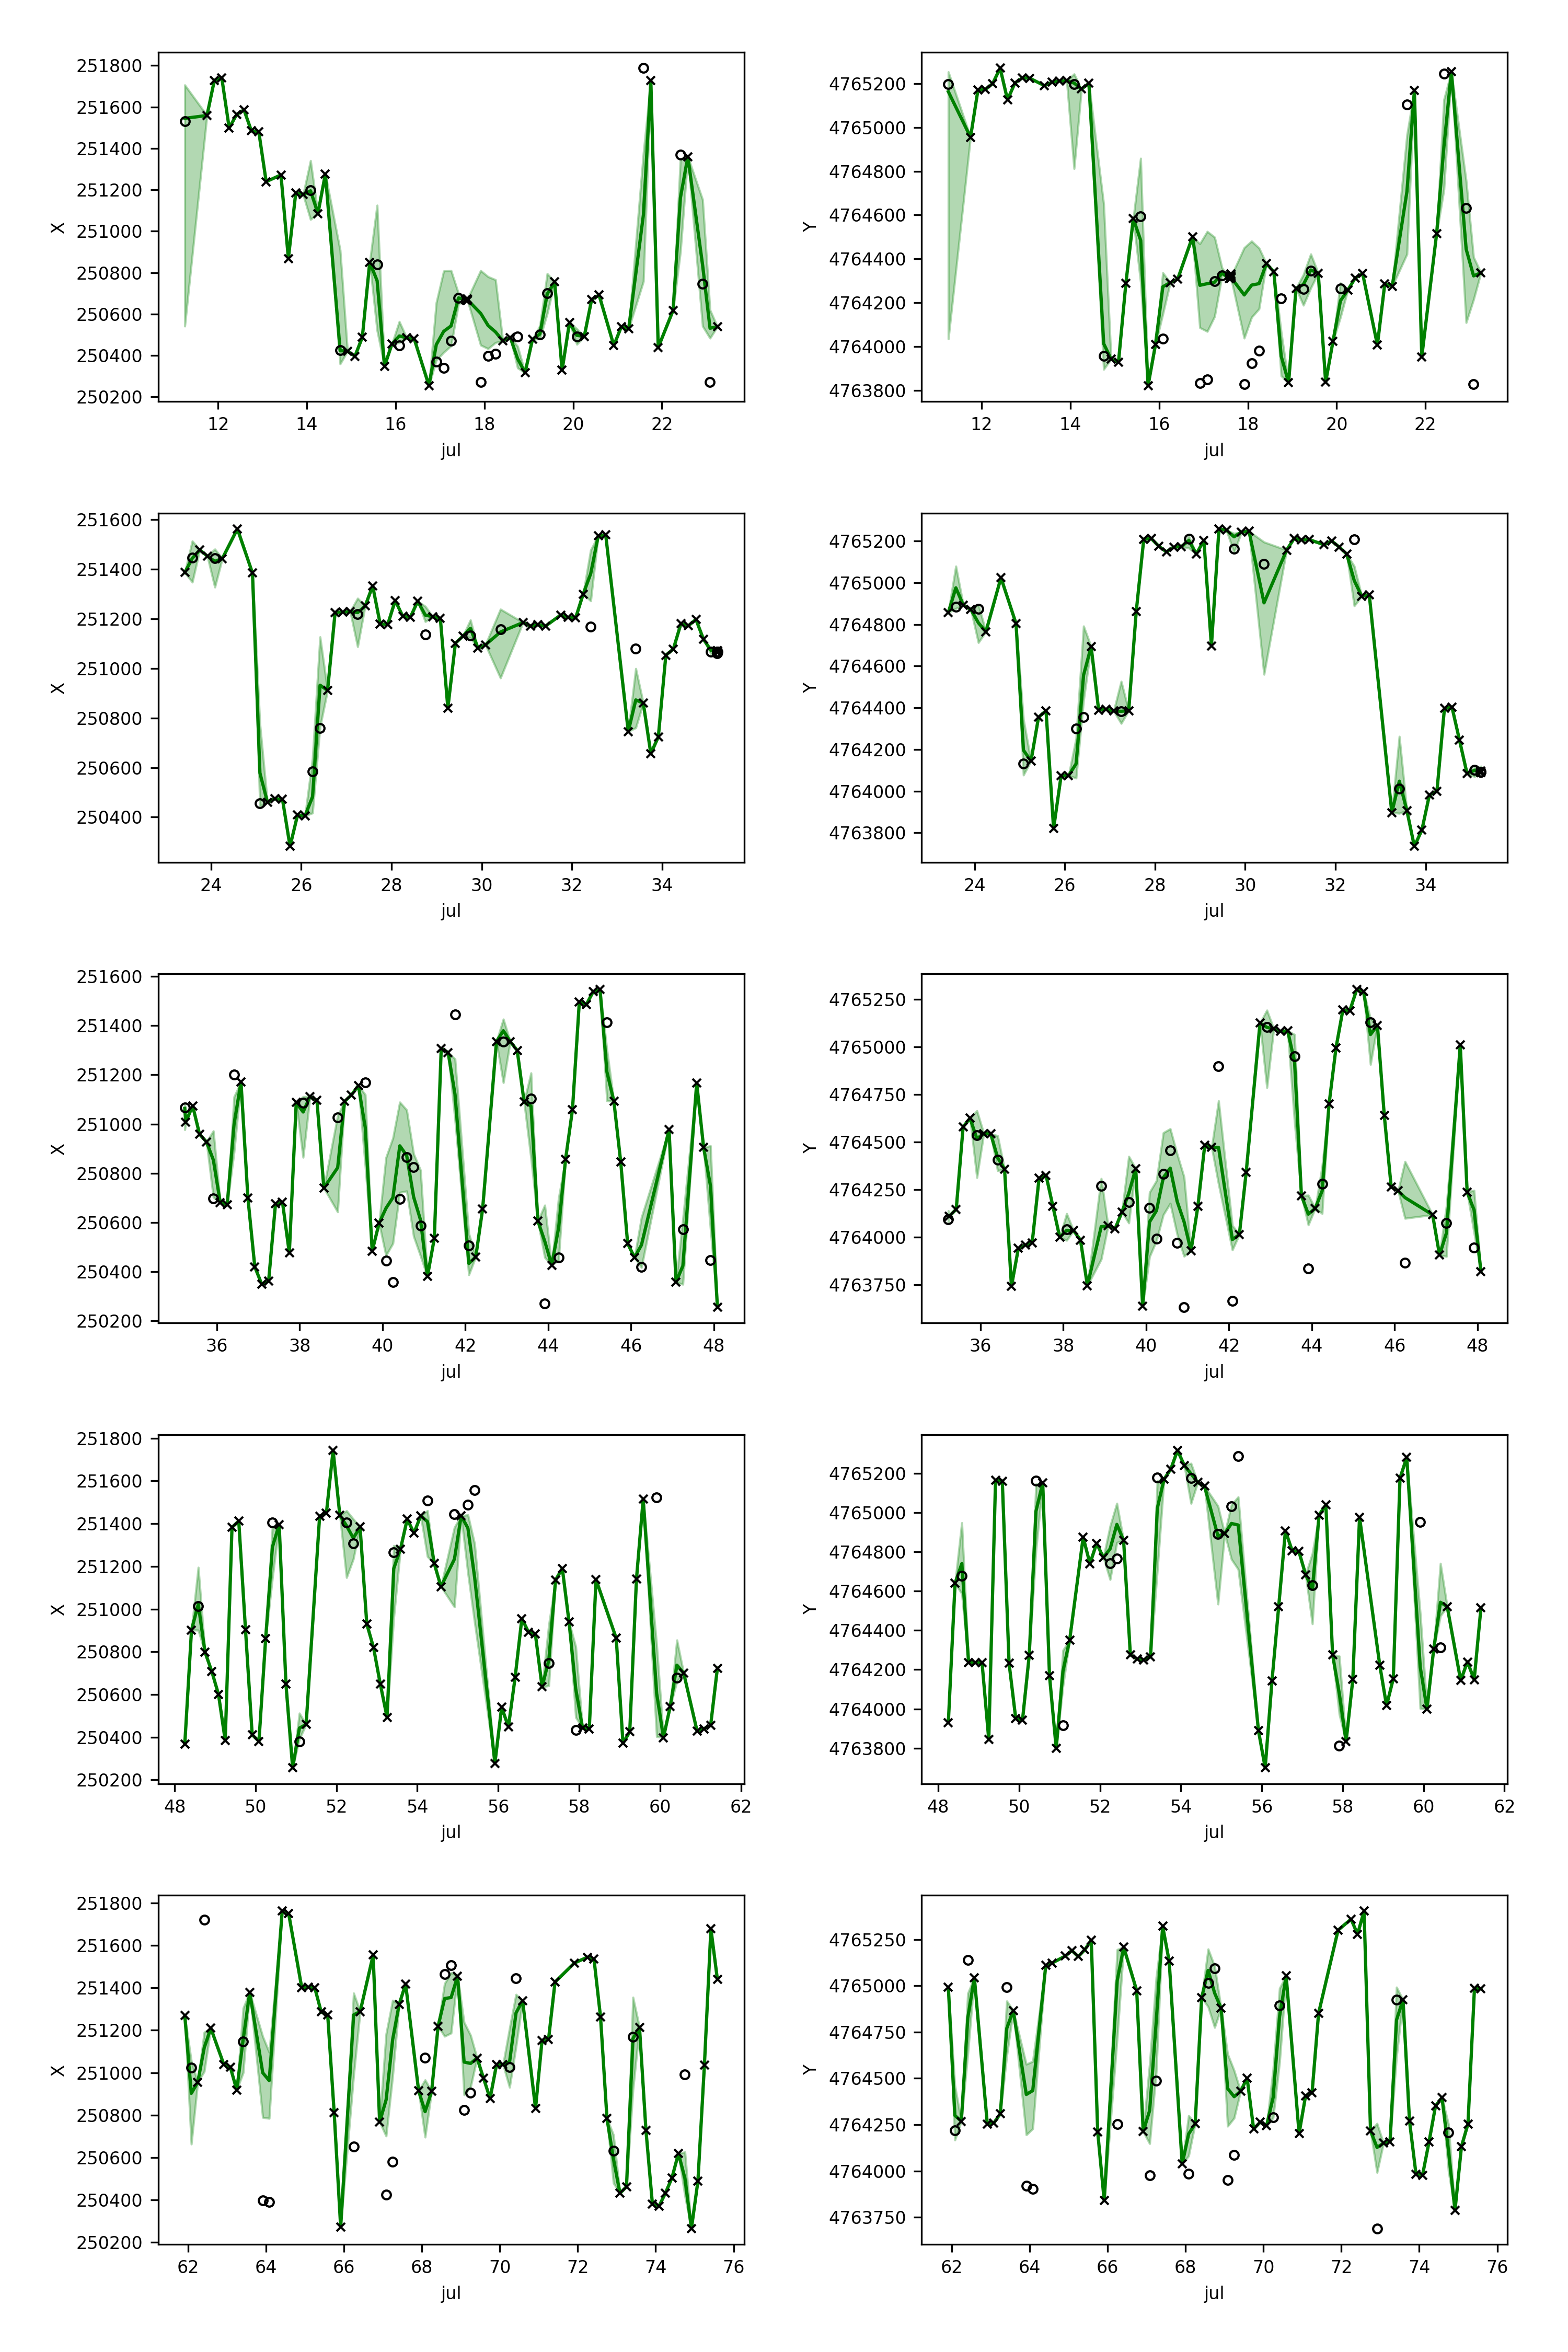
\includegraphics[width=\textwidth]{../figure/20_5094_csdi} % Adjust the scale or width as needed
  \caption{This figure illustrates the imputation results using the CSDI model for a single deer's trajectory with a 20\% missing data ratio. The figure is organized into rows of subplots, with each row showing the deer's trajectory over different time windows. The left subplot in each row shows the X coordinate (longitude) against time (Julian days). The right subplot in each row shows the Y coordinate (latitude) against time. Black ``x" marks represent the observed data points, which are the actual recorded positions of the deer. Unfilled black "o" circles indicate the evaluation data points used for assessing the imputation accuracy. Solid blue lines show the imputed trajectory values generated by the CSDI model. Shaded green areas represent the 95\% confidence interval around the imputed values.}
  \label{fig: csdi_20} % Label for referencing
\end{figure}

\begin{figure}[h]
  \centering
  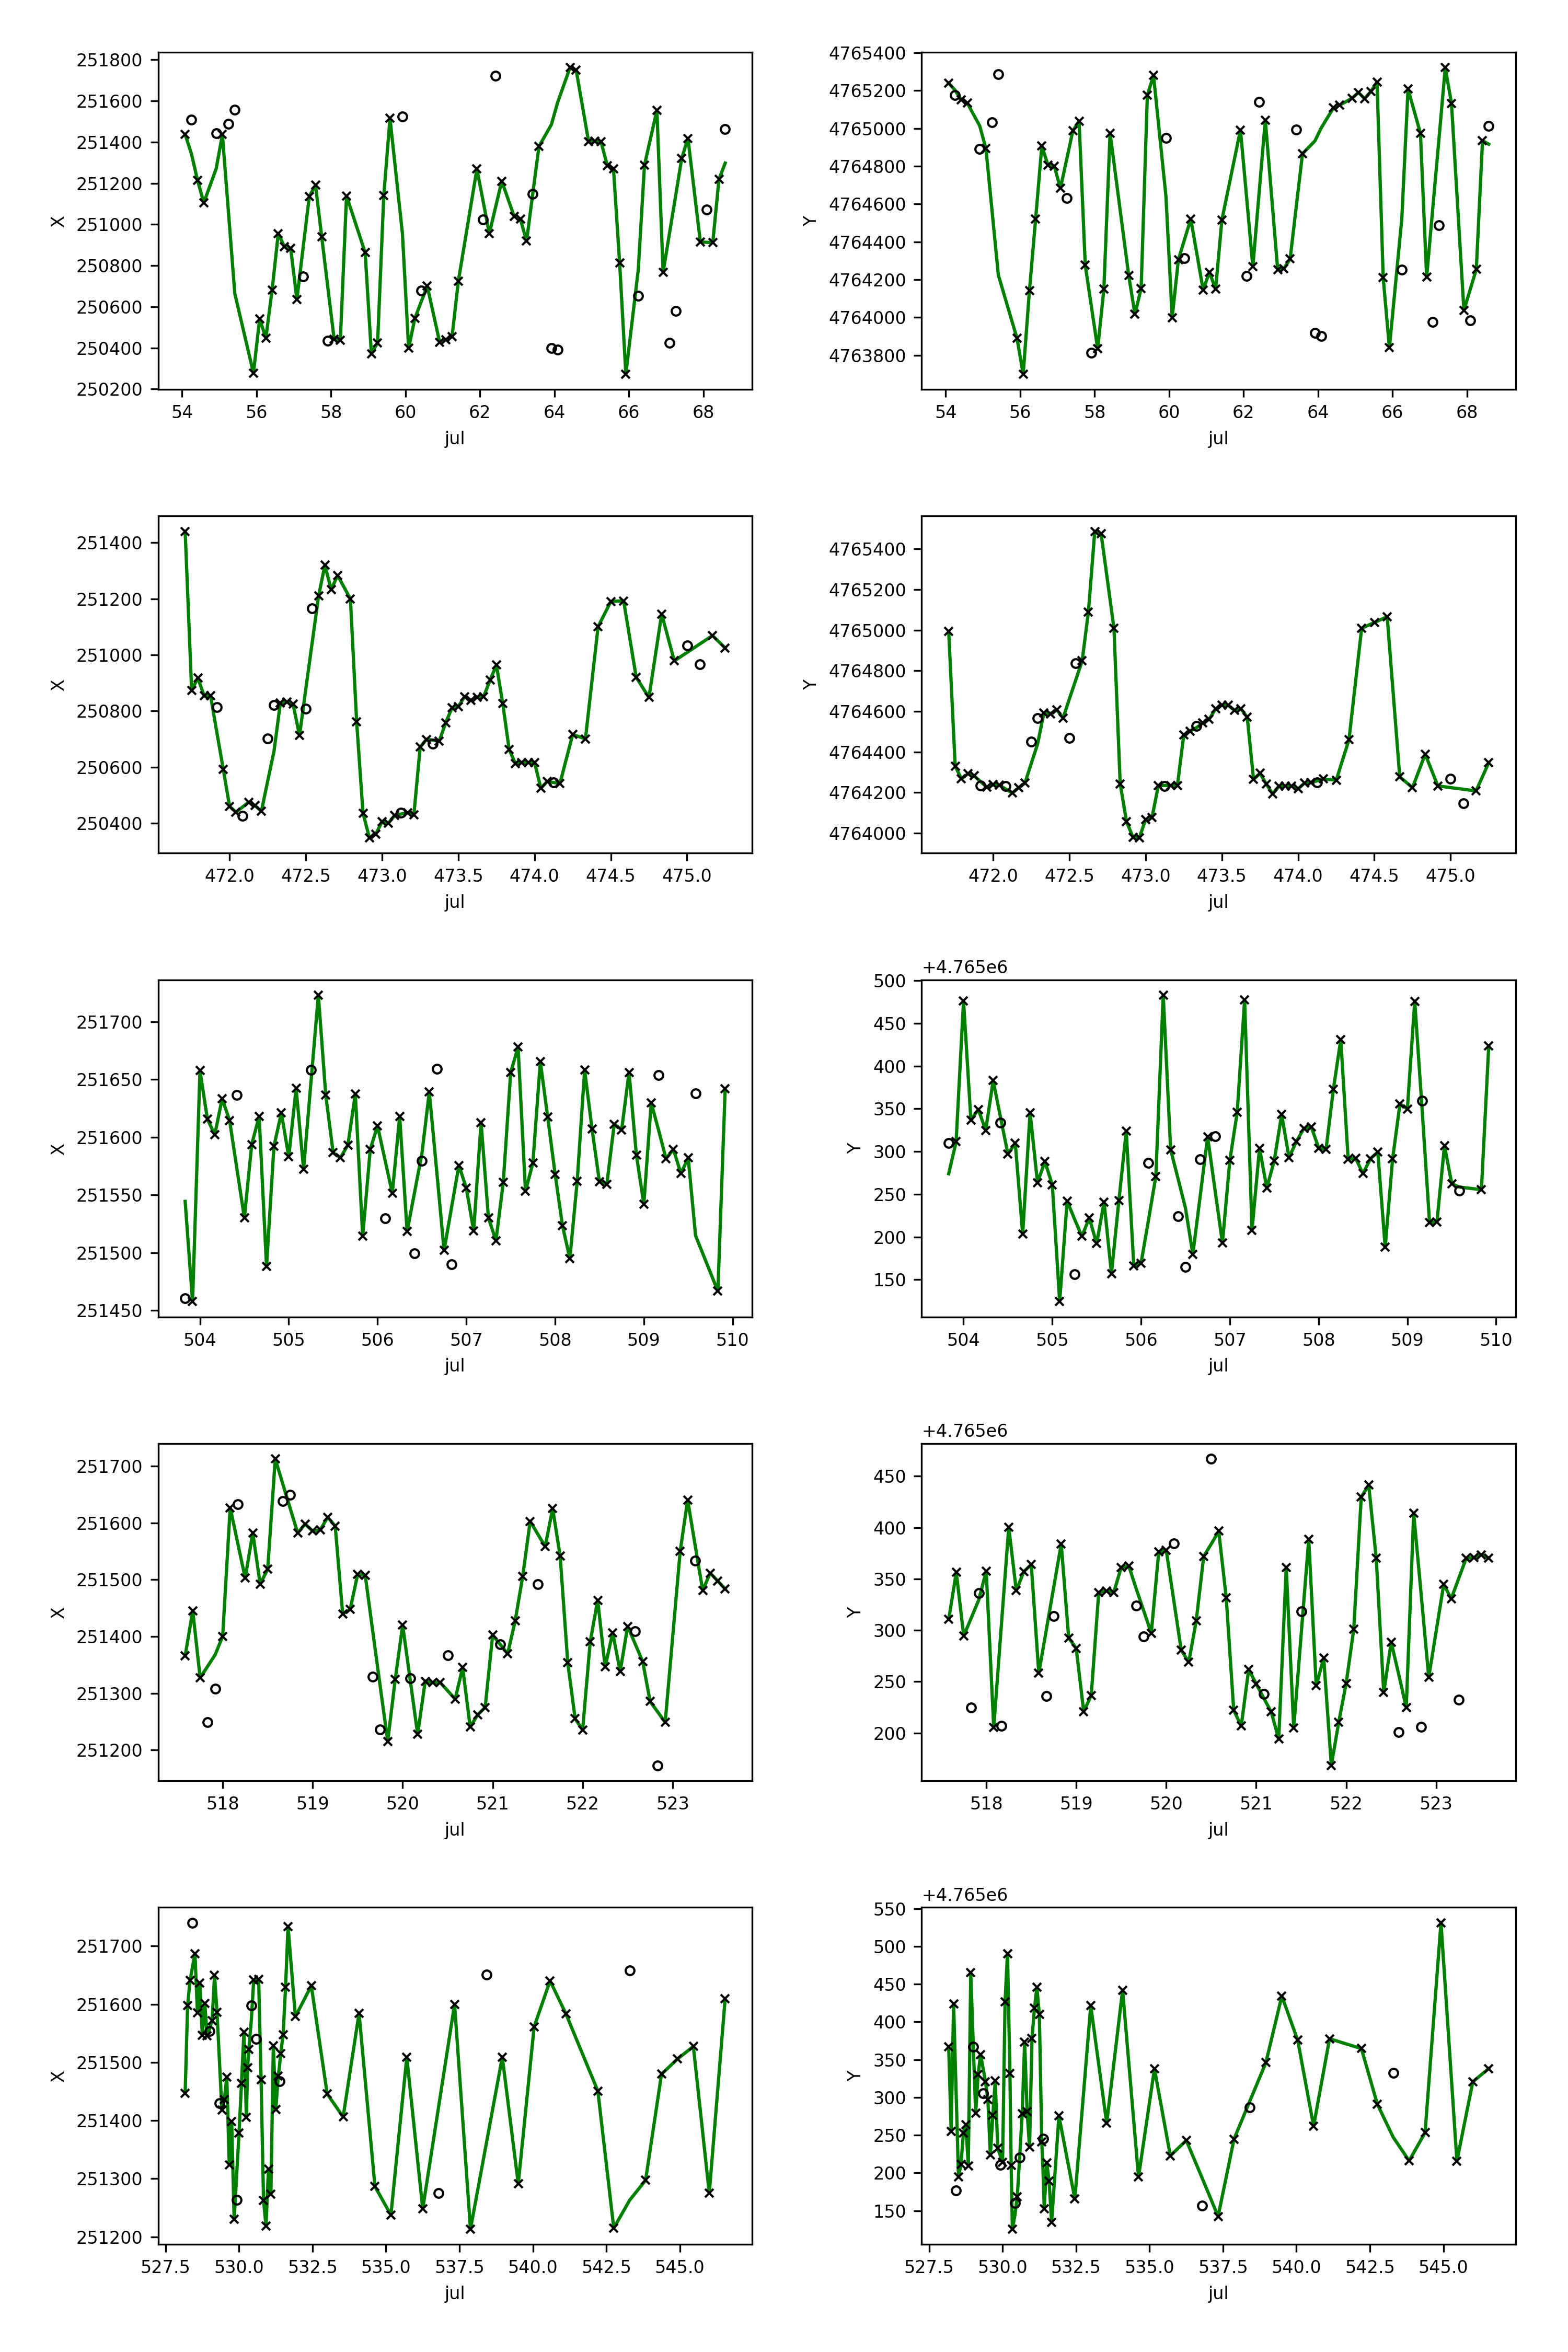
\includegraphics[width=\textwidth]{../figure/20_5094_interpolation} % Adjust the scale or width as needed
  \caption{This figure illustrates the imputation results using interpolation for a single deer's trajectory with a 20\% missing data ratio. The figure is organized into rows of subplots, with each row showing the deer's trajectory over different time windows. The left subplot in each row shows the X coordinate (longitude) against time (Julian days). The right subplot in each row shows the Y coordinate (latitude) against time. Black ``x" marks represent the observed data points, which are the actual recorded positions of the deer. Unfilled black "o" circles indicate the evaluation data points used for assessing the imputation accuracy. Solid blue lines show the imputed trajectory values generated by interpolation.}
  \label{fig: interpolation_20} % Label for referencing
\end{figure}

\begin{figure}[h]
  \centering
  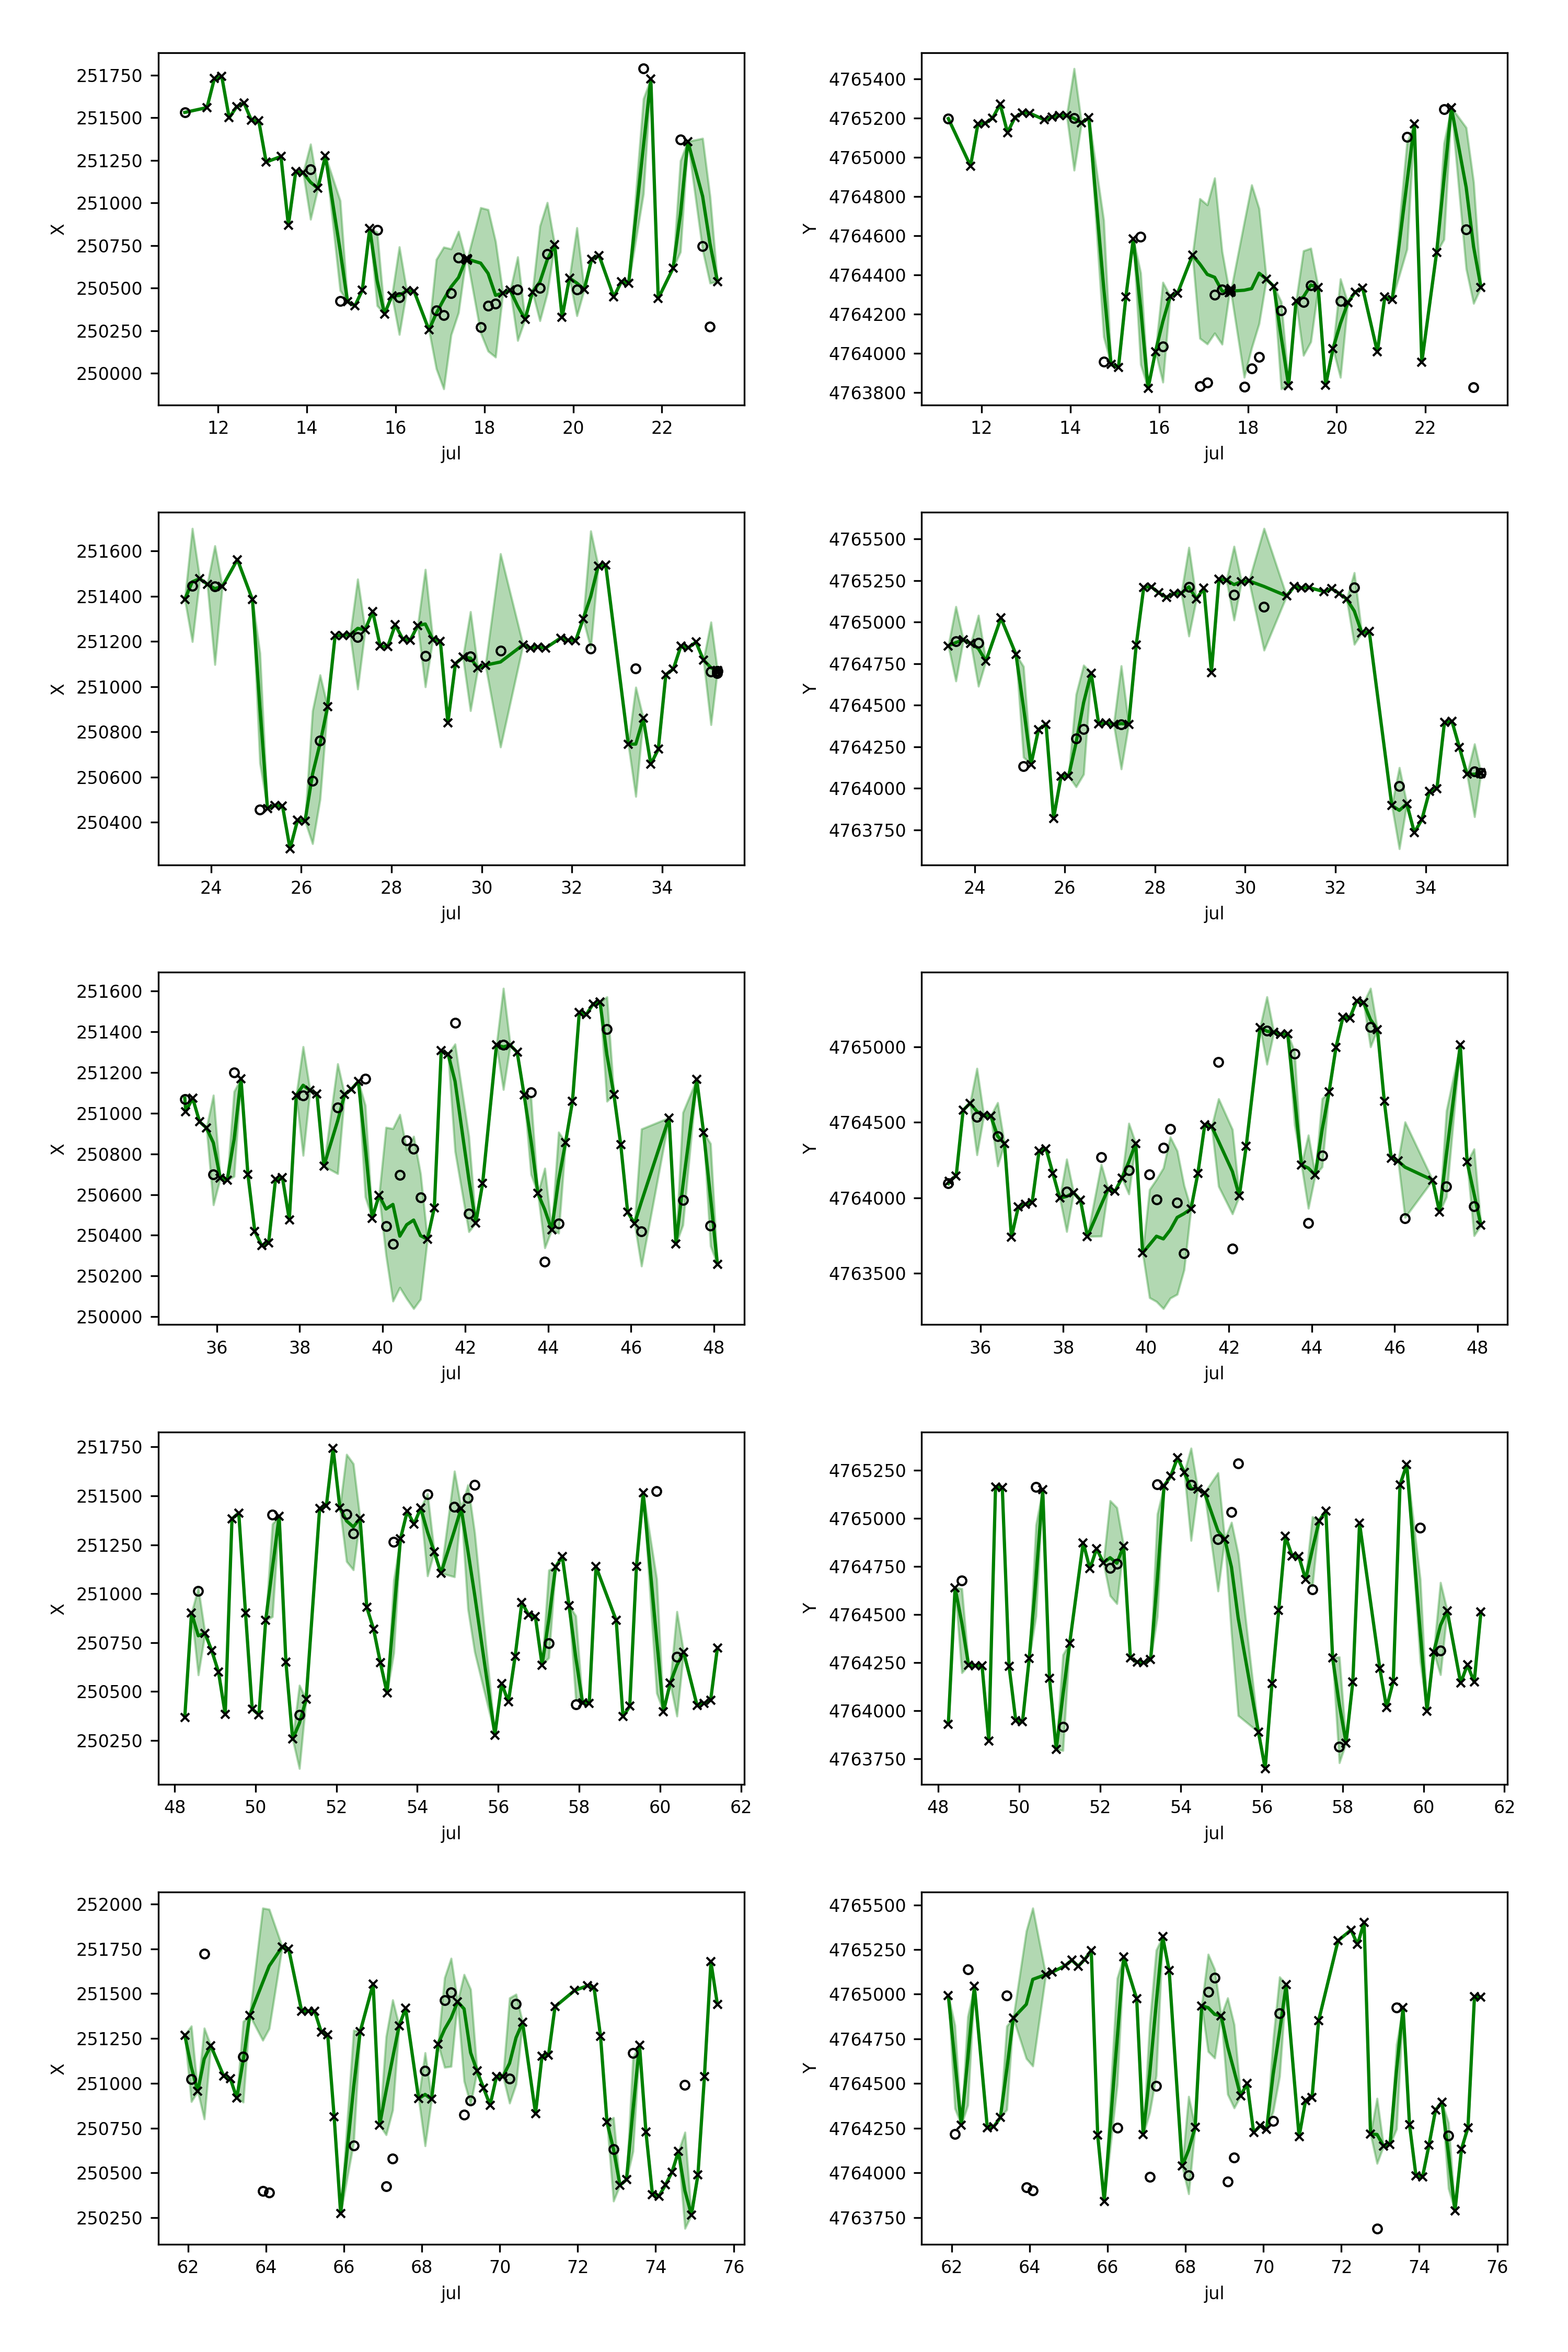
\includegraphics[width=\textwidth]{../figure/20_5094_crawl} % Adjust the scale or width as needed
  \caption{This figure illustrates the imputation results using the Continuous-Time Correlated Random Walk (CTCRW) model for a single deer's trajectory with a 20\% missing data ratio. The figure is organized into rows of subplots, with each row showing the deer's trajectory over different time windows. The left subplot in each row shows the X coordinate (longitude) against time (Julian days). The right subplot in each row shows the Y coordinate (latitude) against time. Black ``x" marks represent the observed data points, which are the actual recorded positions of the deer. Unfilled black "o" circles indicate the evaluation data points used for assessing the imputation accuracy. Solid blue lines show the imputed trajectory values generated by the CTCRW model. Shaded green areas represent the 95\% confidence interval around the imputed values.
}
  \label{fig: ctcrw_20} % Label for referencing
\end{figure}


\begin{figure}[h]
  \centering
  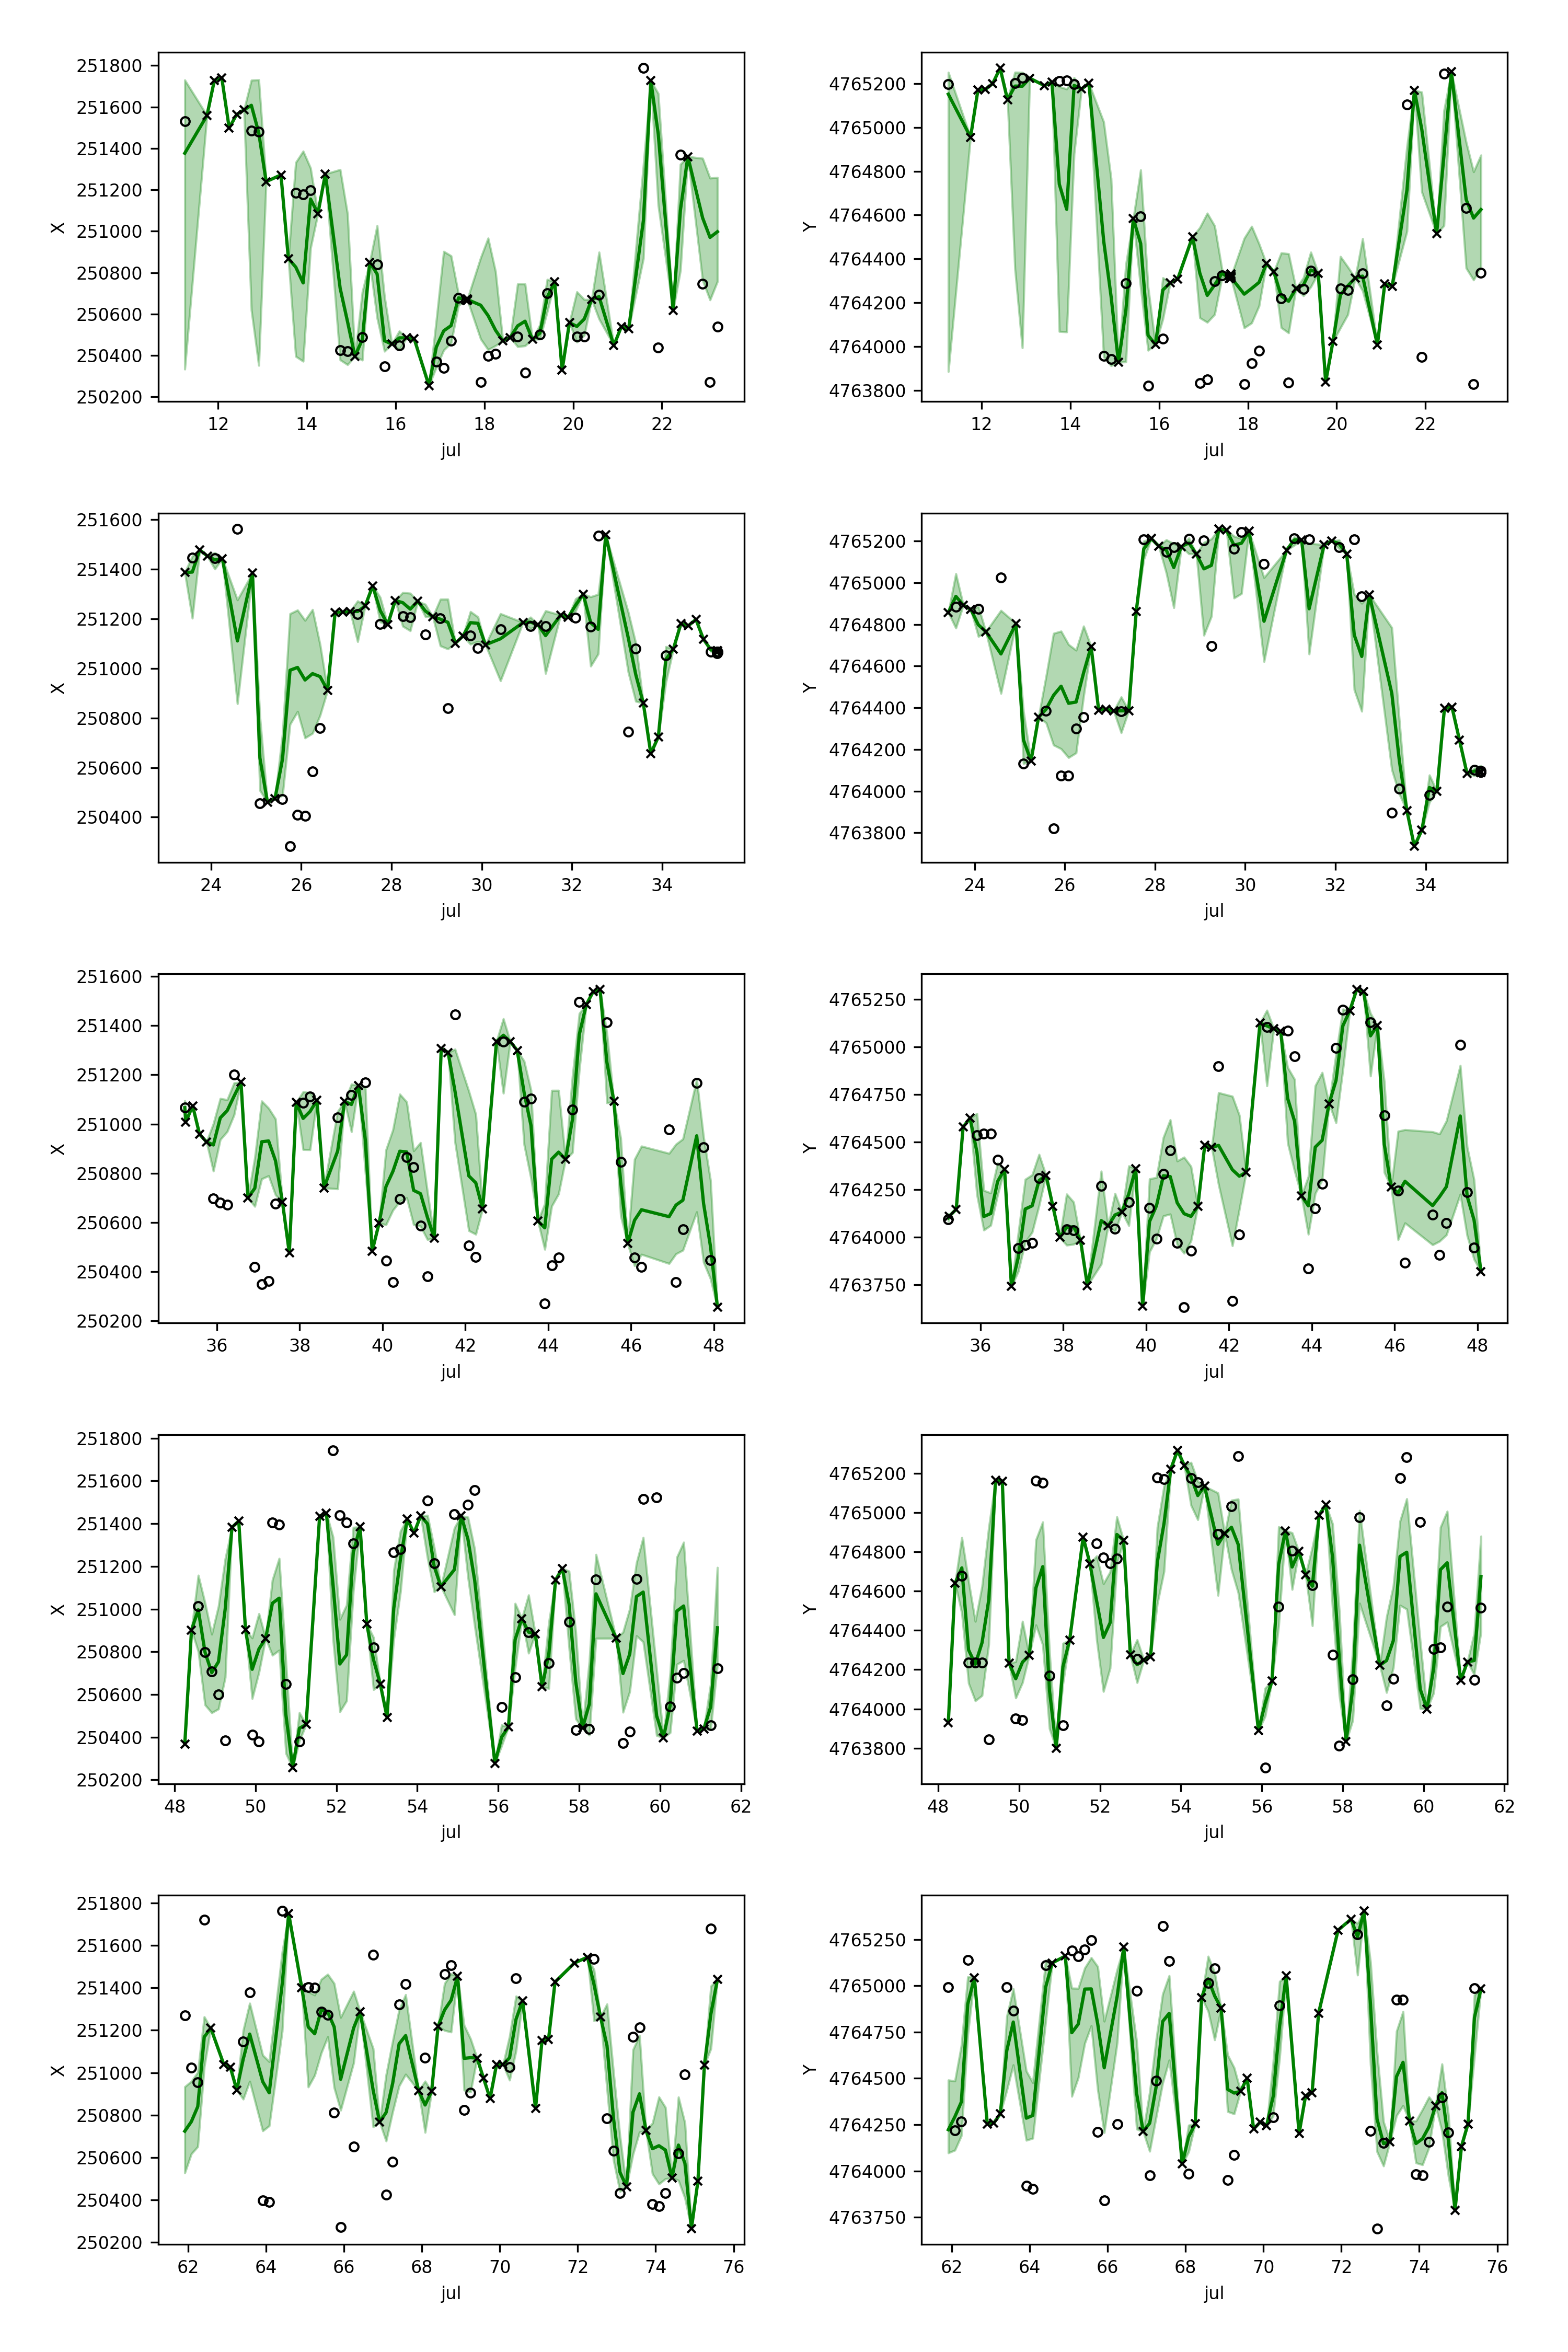
\includegraphics[width=\textwidth]{../figure/50_5094_csdi} % Adjust the scale or width as needed
  \caption{This figure illustrates the imputation results using the CSDI model for a single deer's trajectory with a 50\% missing data ratio. The figure is organized into rows of subplots, with each row showing the deer's trajectory over different time windows. The left subplot in each row shows the X coordinate (longitude) against time (Julian days). The right subplot in each row shows the Y coordinate (latitude) against time. Black ``x" marks represent the observed data points, which are the actual recorded positions of the deer. Unfilled black "o" circles indicate the evaluation data points used for assessing the imputation accuracy. Solid blue lines show the imputed trajectory values generated by the CSDI model. Shaded green areas represent the 95\% confidence interval around the imputed values.}
  \label{fig: csdi_50} % Label for referencing
\end{figure}

\begin{figure}[h]
  \centering
  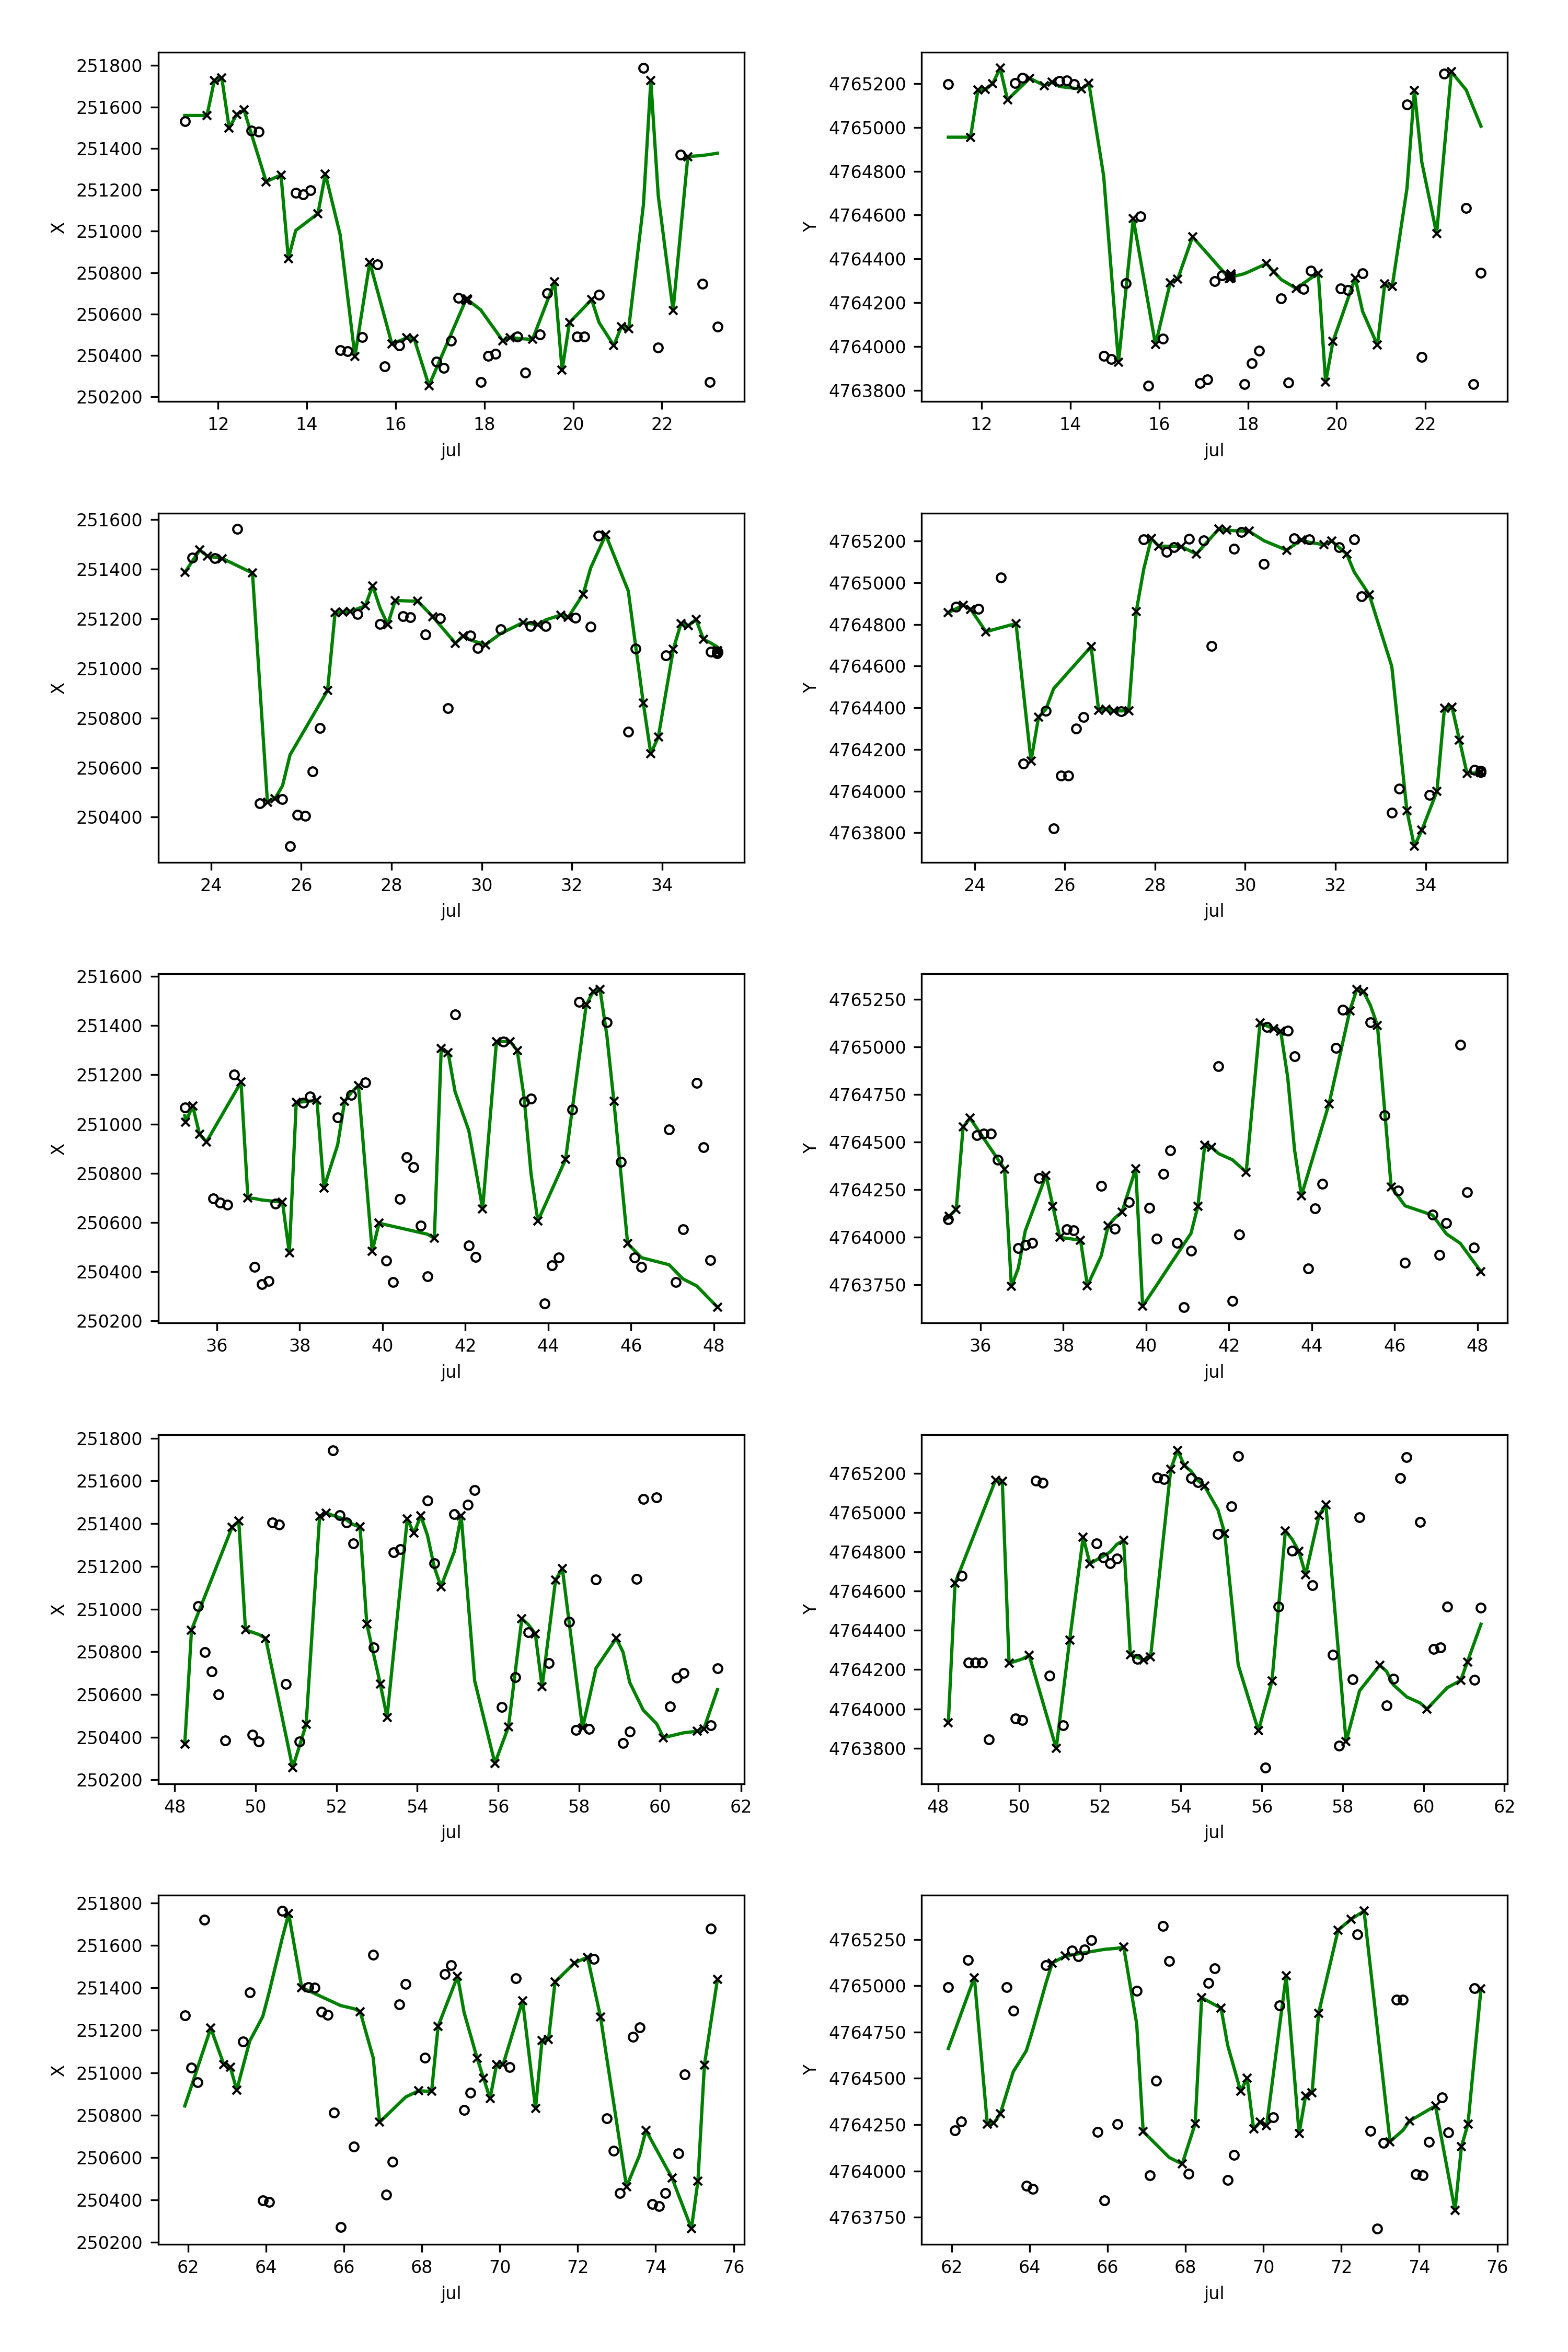
\includegraphics[width=\textwidth]{../figure/50_5094_interpolation} % Adjust the scale or width as needed
  \caption{This figure illustrates the imputation results using interpolation for a single deer's trajectory with a 50\% missing data ratio. The figure is organized into rows of subplots, with each row showing the deer's trajectory over different time windows. The left subplot in each row shows the X coordinate (longitude) against time (Julian days). The right subplot in each row shows the Y coordinate (latitude) against time. Black ``x" marks represent the observed data points, which are the actual recorded positions of the deer. Unfilled black "o" circles indicate the evaluation data points used for assessing the imputation accuracy. Solid blue lines show the imputed trajectory values generated by interpolation.}
  \label{fig: interpolation_50} % Label for referencing
\end{figure}

\begin{figure}[h]
  \centering
  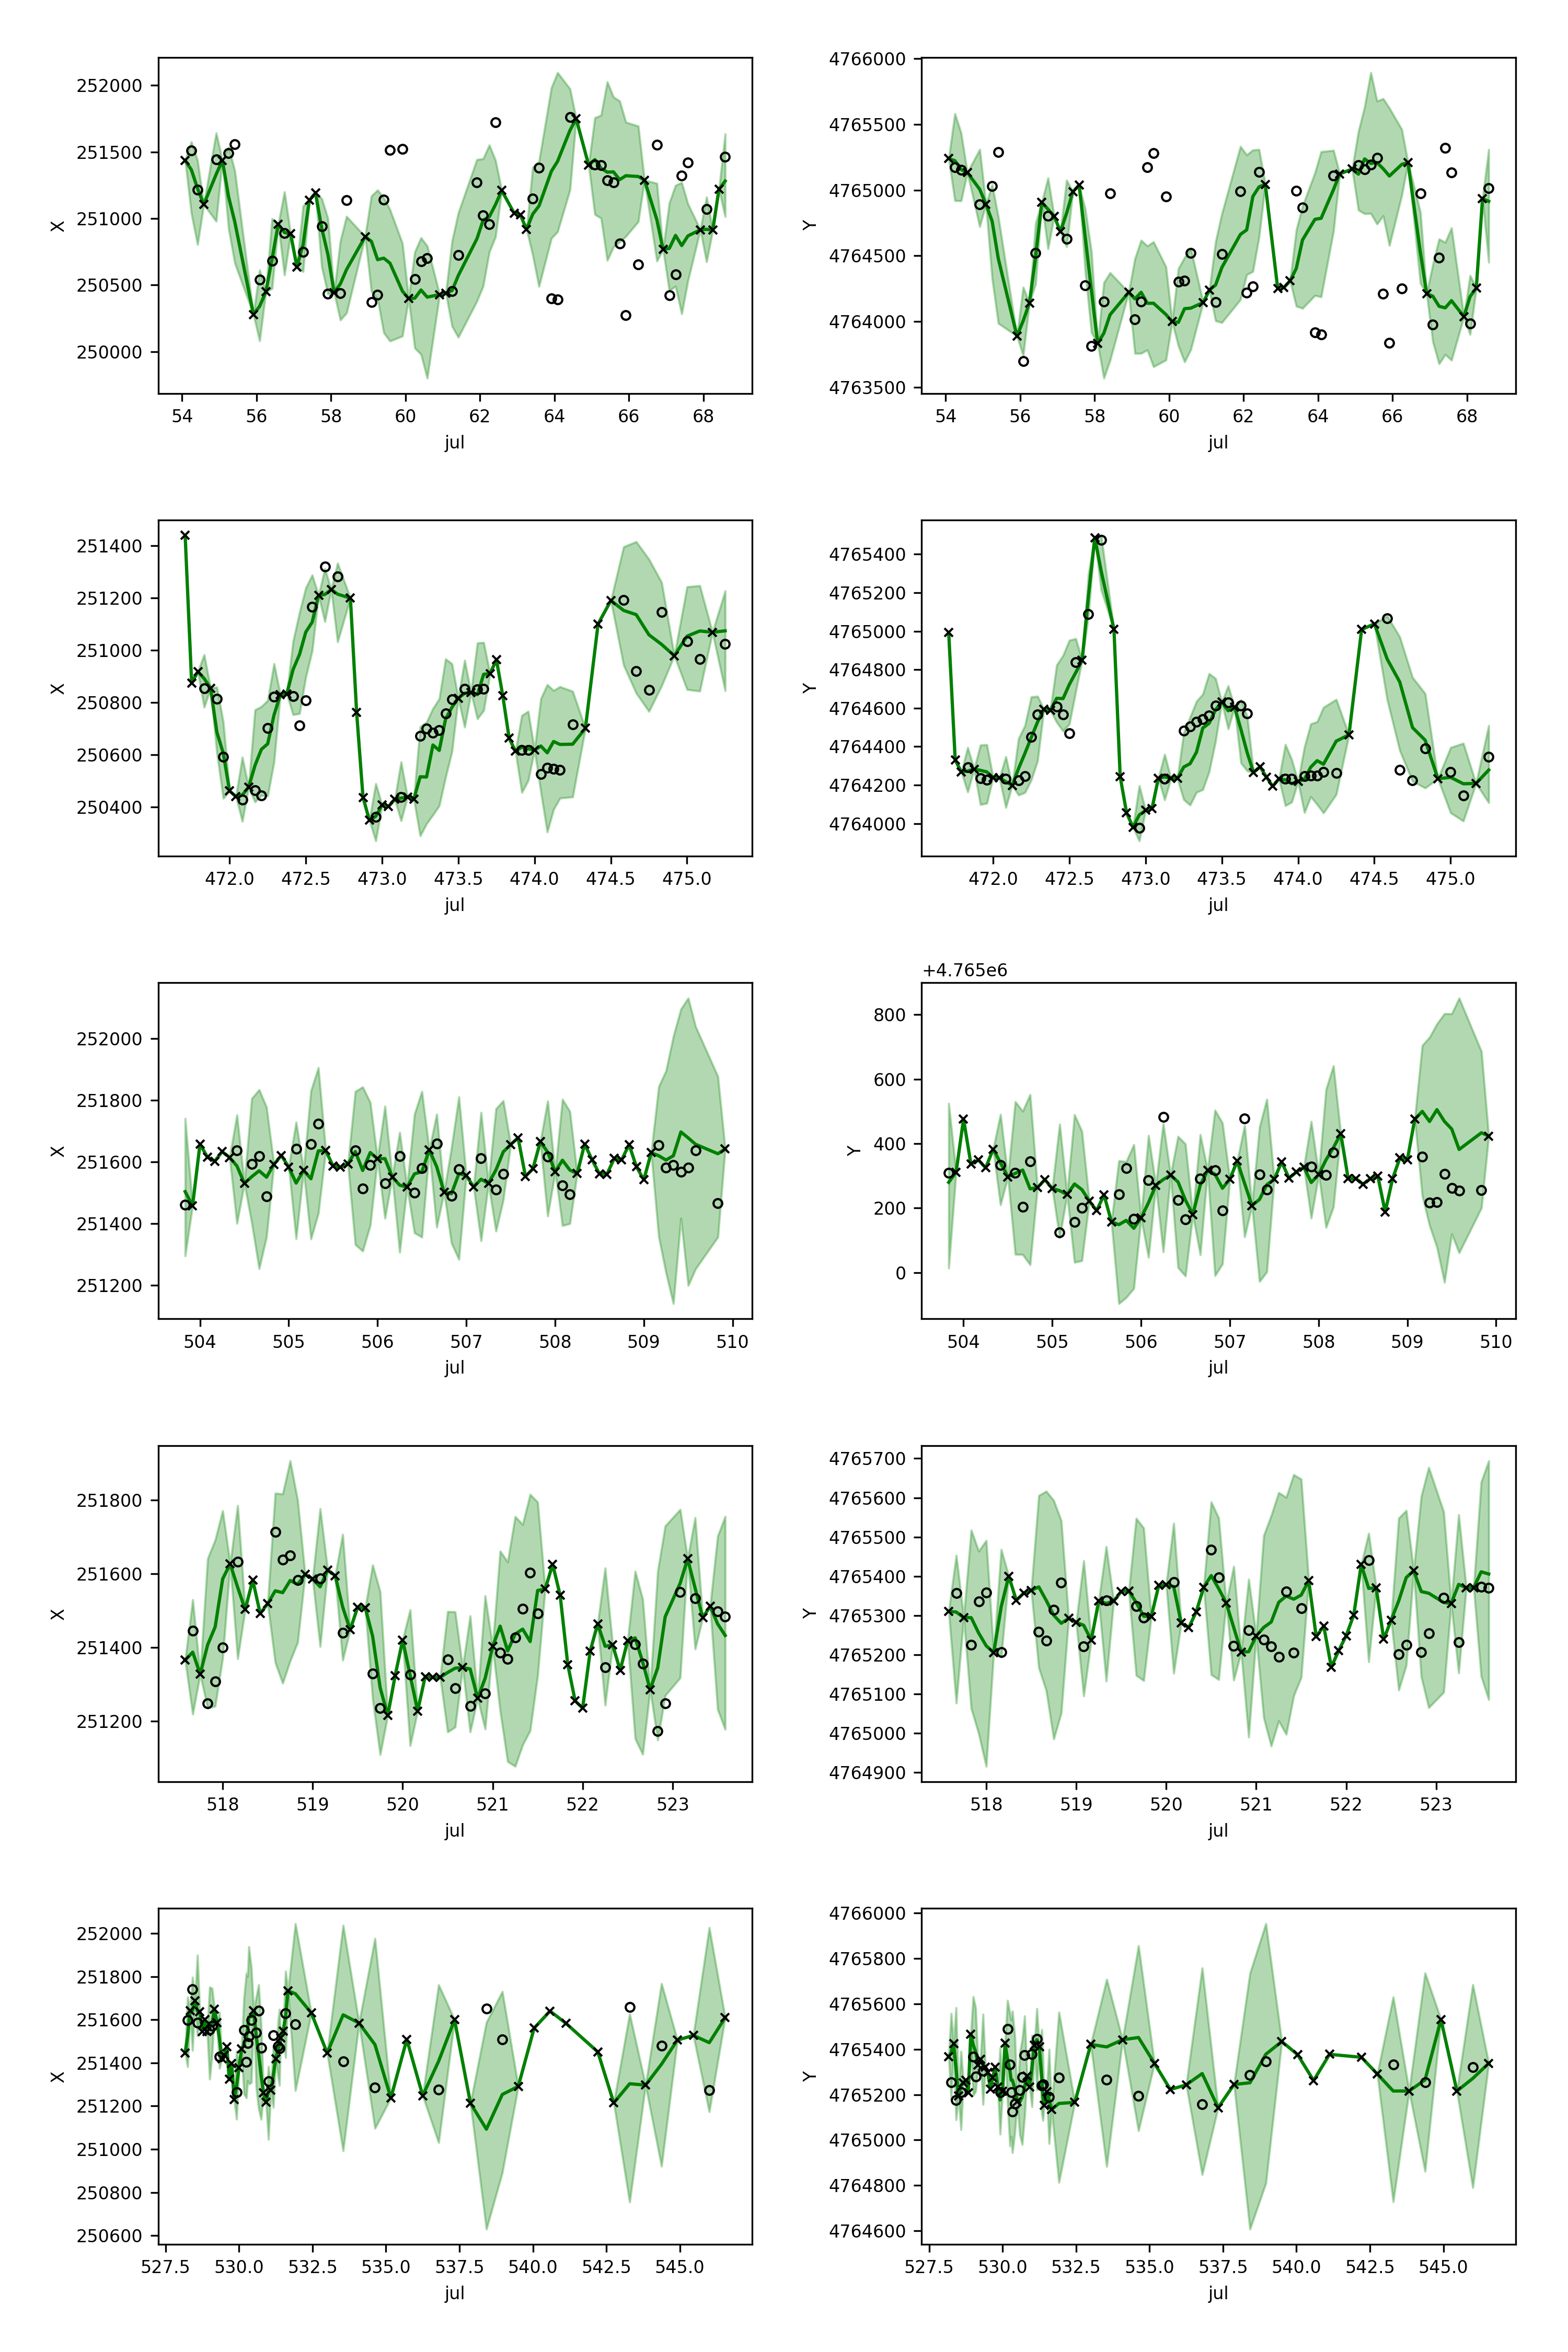
\includegraphics[width=\textwidth]{../figure/50_5094_crawl} % Adjust the scale or width as needed
  \caption{This figure illustrates the imputation results using the Continuous-Time Correlated Random Walk (CTCRW) model for a single deer's trajectory with a 50\% missing data ratio. The figure is organized into rows of subplots, with each row showing the deer's trajectory over different time windows. The left subplot in each row shows the X coordinate (longitude) against time (Julian days). The right subplot in each row shows the Y coordinate (latitude) against time. Black ``x" marks represent the observed data points, which are the actual recorded positions of the deer. Unfilled black "o" circles indicate the evaluation data points used for assessing the imputation accuracy. Solid blue lines show the imputed trajectory values generated by the CTCRW model. Shaded green areas represent the 95\% confidence interval around the imputed values.}
  \label{fig: ctcrw_50} % Label for referencing
\end{figure}

\begin{figure}[h]
  \centering
  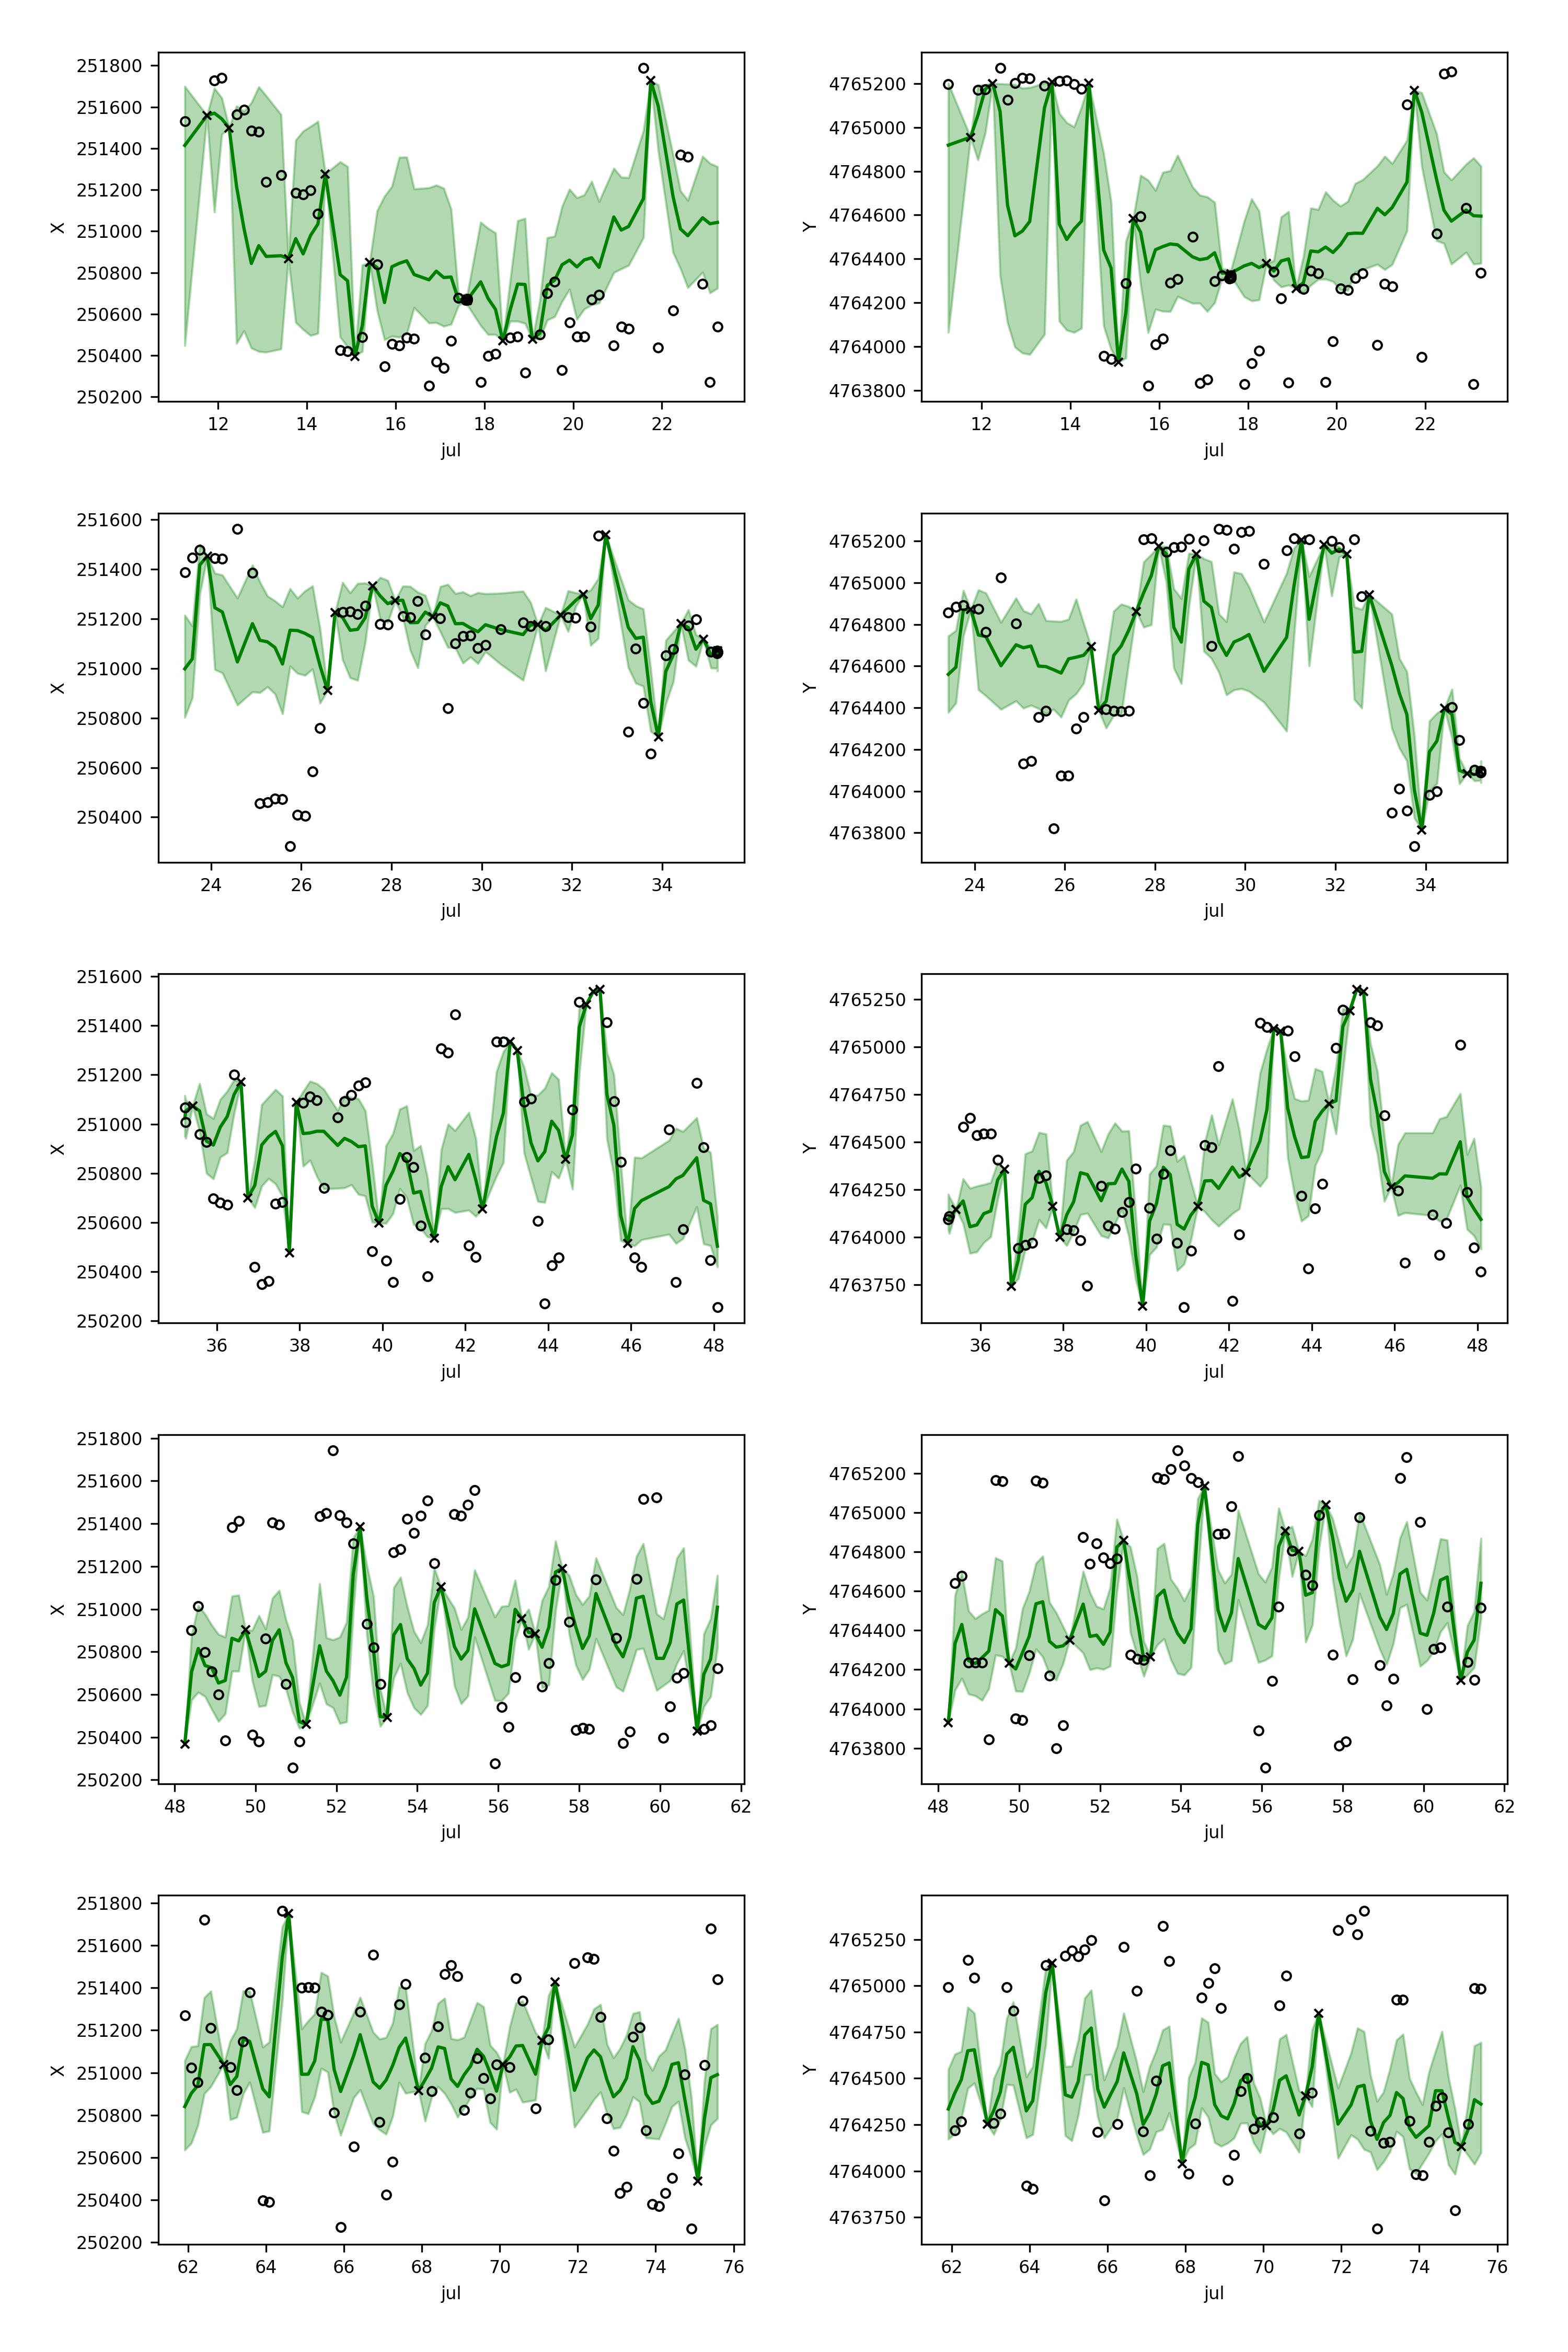
\includegraphics[width=\textwidth]{../figure/80_5094_csdi} % Adjust the scale or width as needed
  \caption{This figure illustrates the imputation results using the CSDI model for a single deer's trajectory with a 80\% missing data ratio. The figure is organized into rows of subplots, with each row showing the deer's trajectory over different time windows. The left subplot in each row shows the X coordinate (longitude) against time (Julian days). The right subplot in each row shows the Y coordinate (latitude) against time. Black ``x" marks represent the observed data points, which are the actual recorded positions of the deer. Unfilled black "o" circles indicate the evaluation data points used for assessing the imputation accuracy. Solid blue lines show the imputed trajectory values generated by the CSDI model. Shaded green areas represent the 95\% confidence interval around the imputed values.}
  \label{fig: csdi_80} % Label for referencing
\end{figure}

\begin{figure}[h]
  \centering
  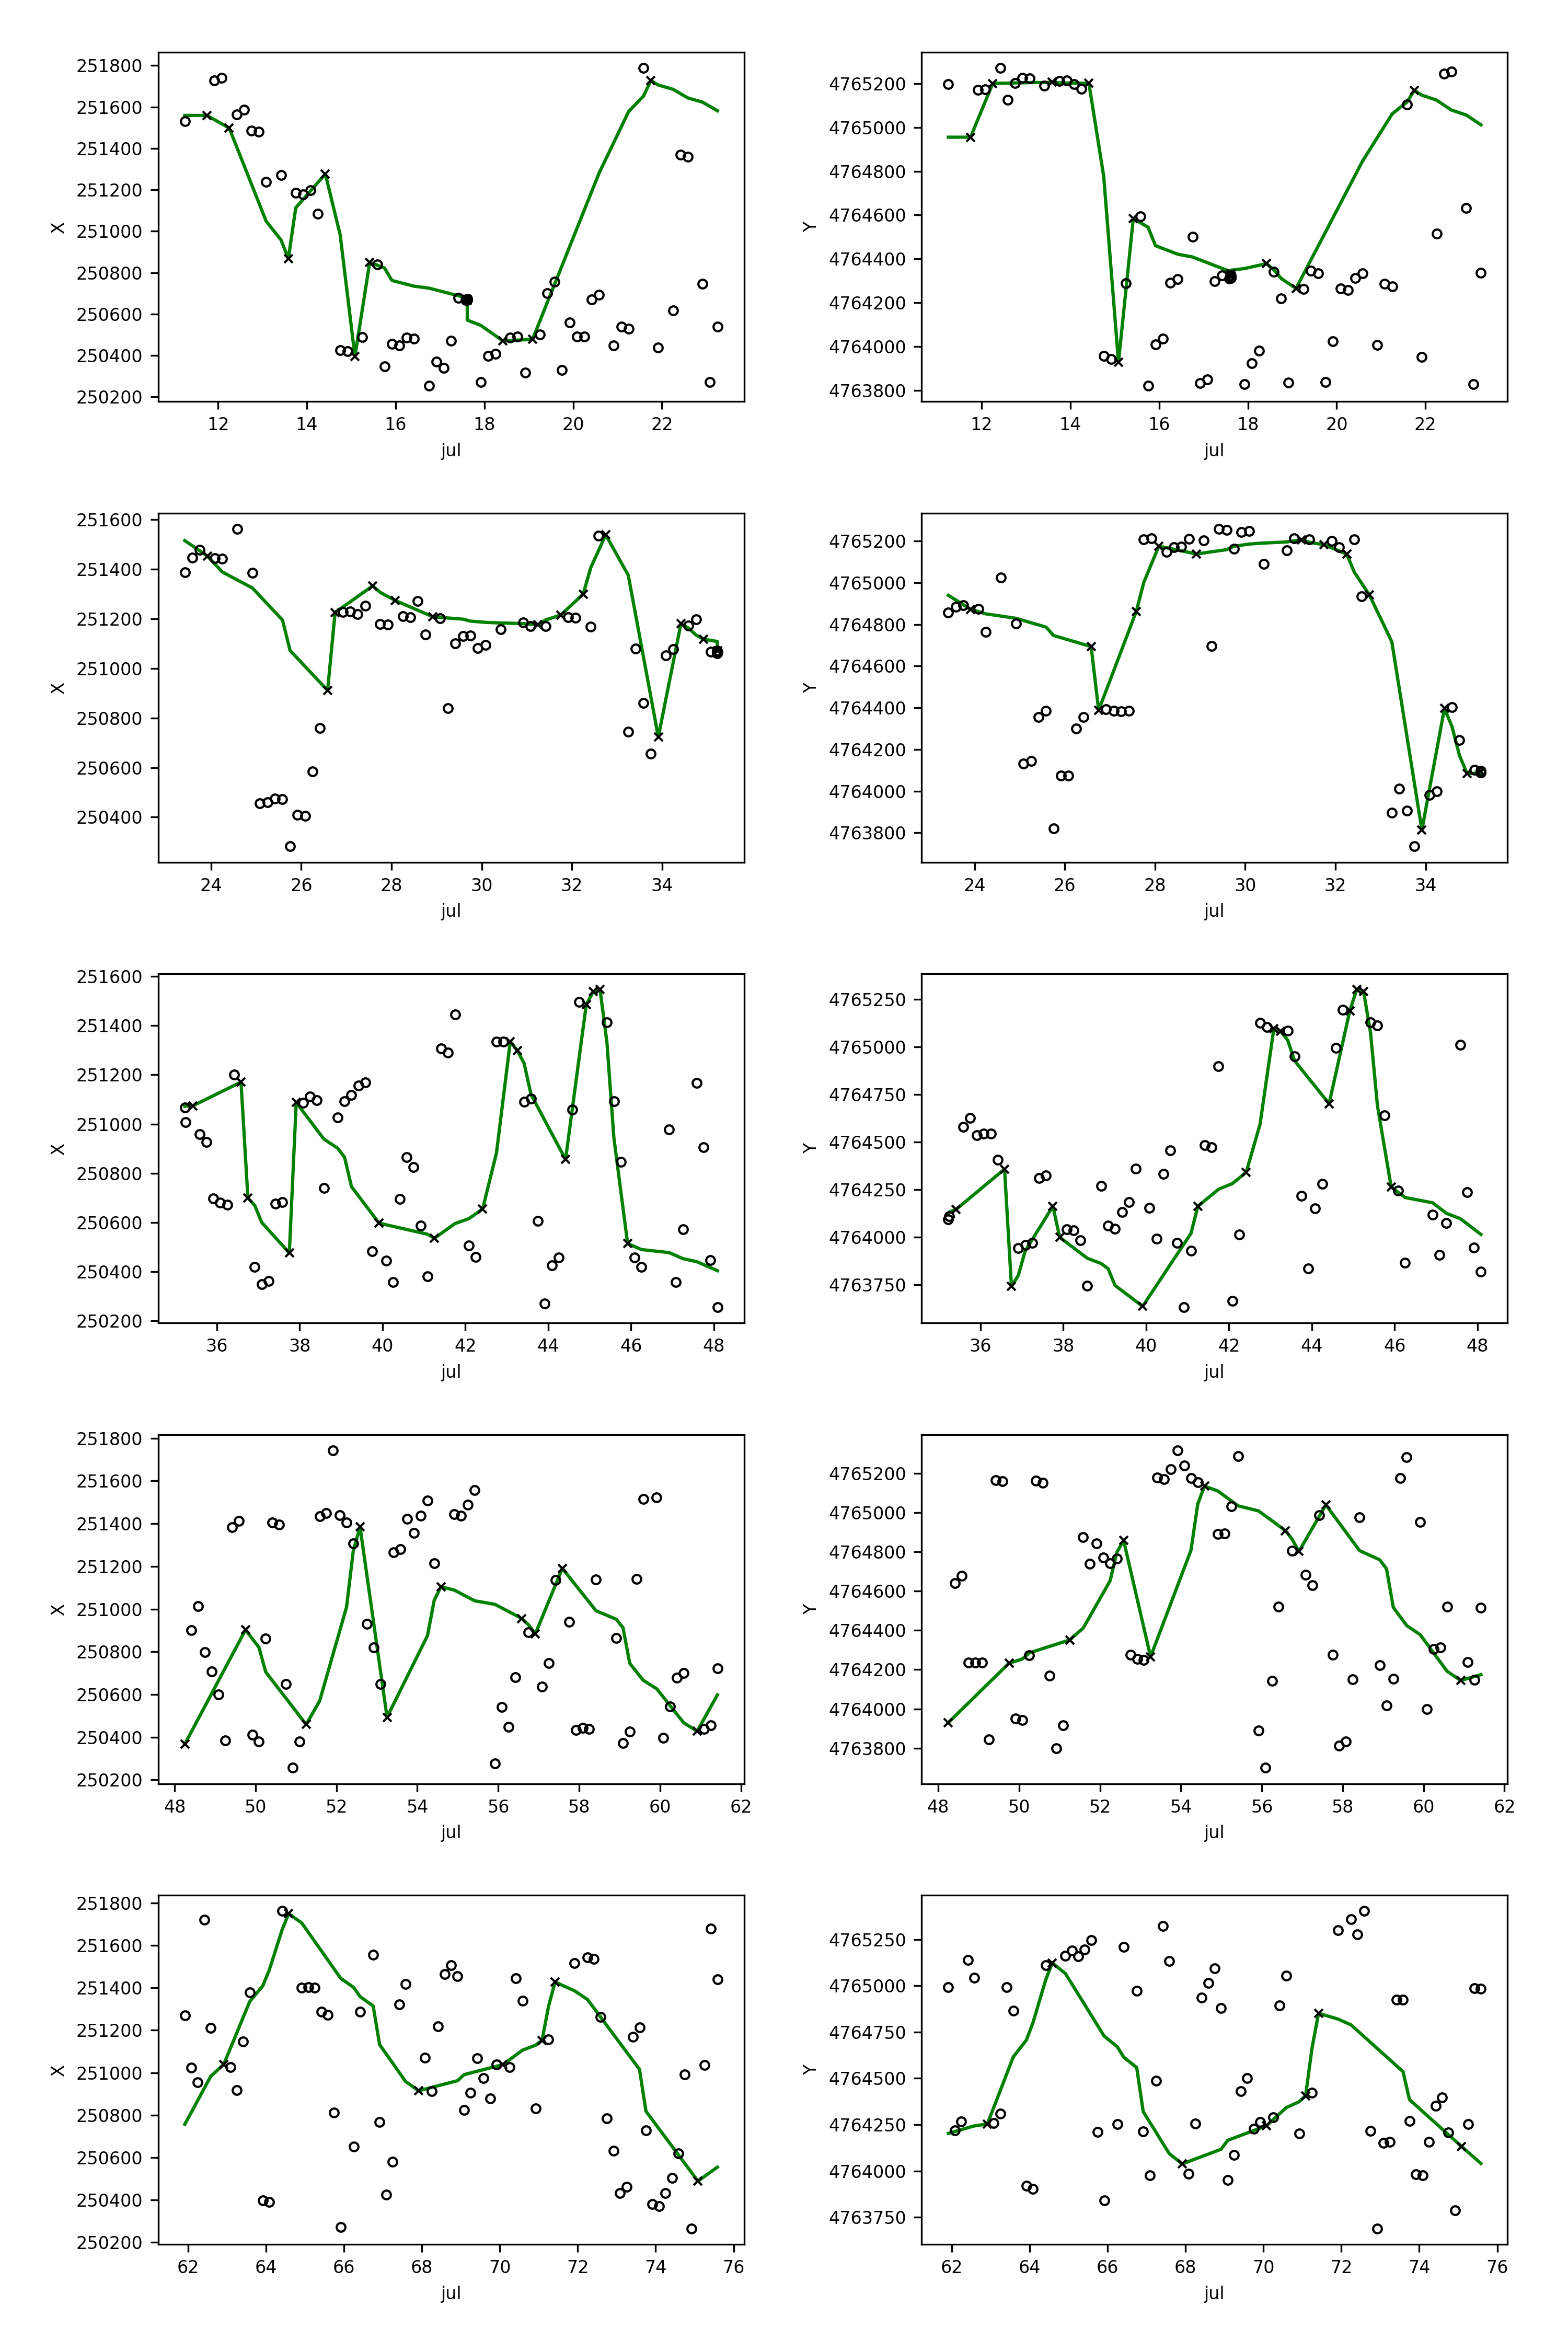
\includegraphics[width=\textwidth]{../figure/80_5094_interpolation} % Adjust the scale or width as needed
  \caption{This figure illustrates the imputation results using interpolation for a single deer's trajectory with a 80\% missing data ratio. The figure is organized into rows of subplots, with each row showing the deer's trajectory over different time windows. The left subplot in each row shows the X coordinate (longitude) against time (Julian days). The right subplot in each row shows the Y coordinate (latitude) against time. Black ``x" marks represent the observed data points, which are the actual recorded positions of the deer. Unfilled black "o" circles indicate the evaluation data points used for assessing the imputation accuracy. Solid blue lines show the imputed trajectory values generated by interpolation.}
  \label{fig: interpolation_80} % Label for referencing
\end{figure}

\begin{figure}[h]
  \centering
  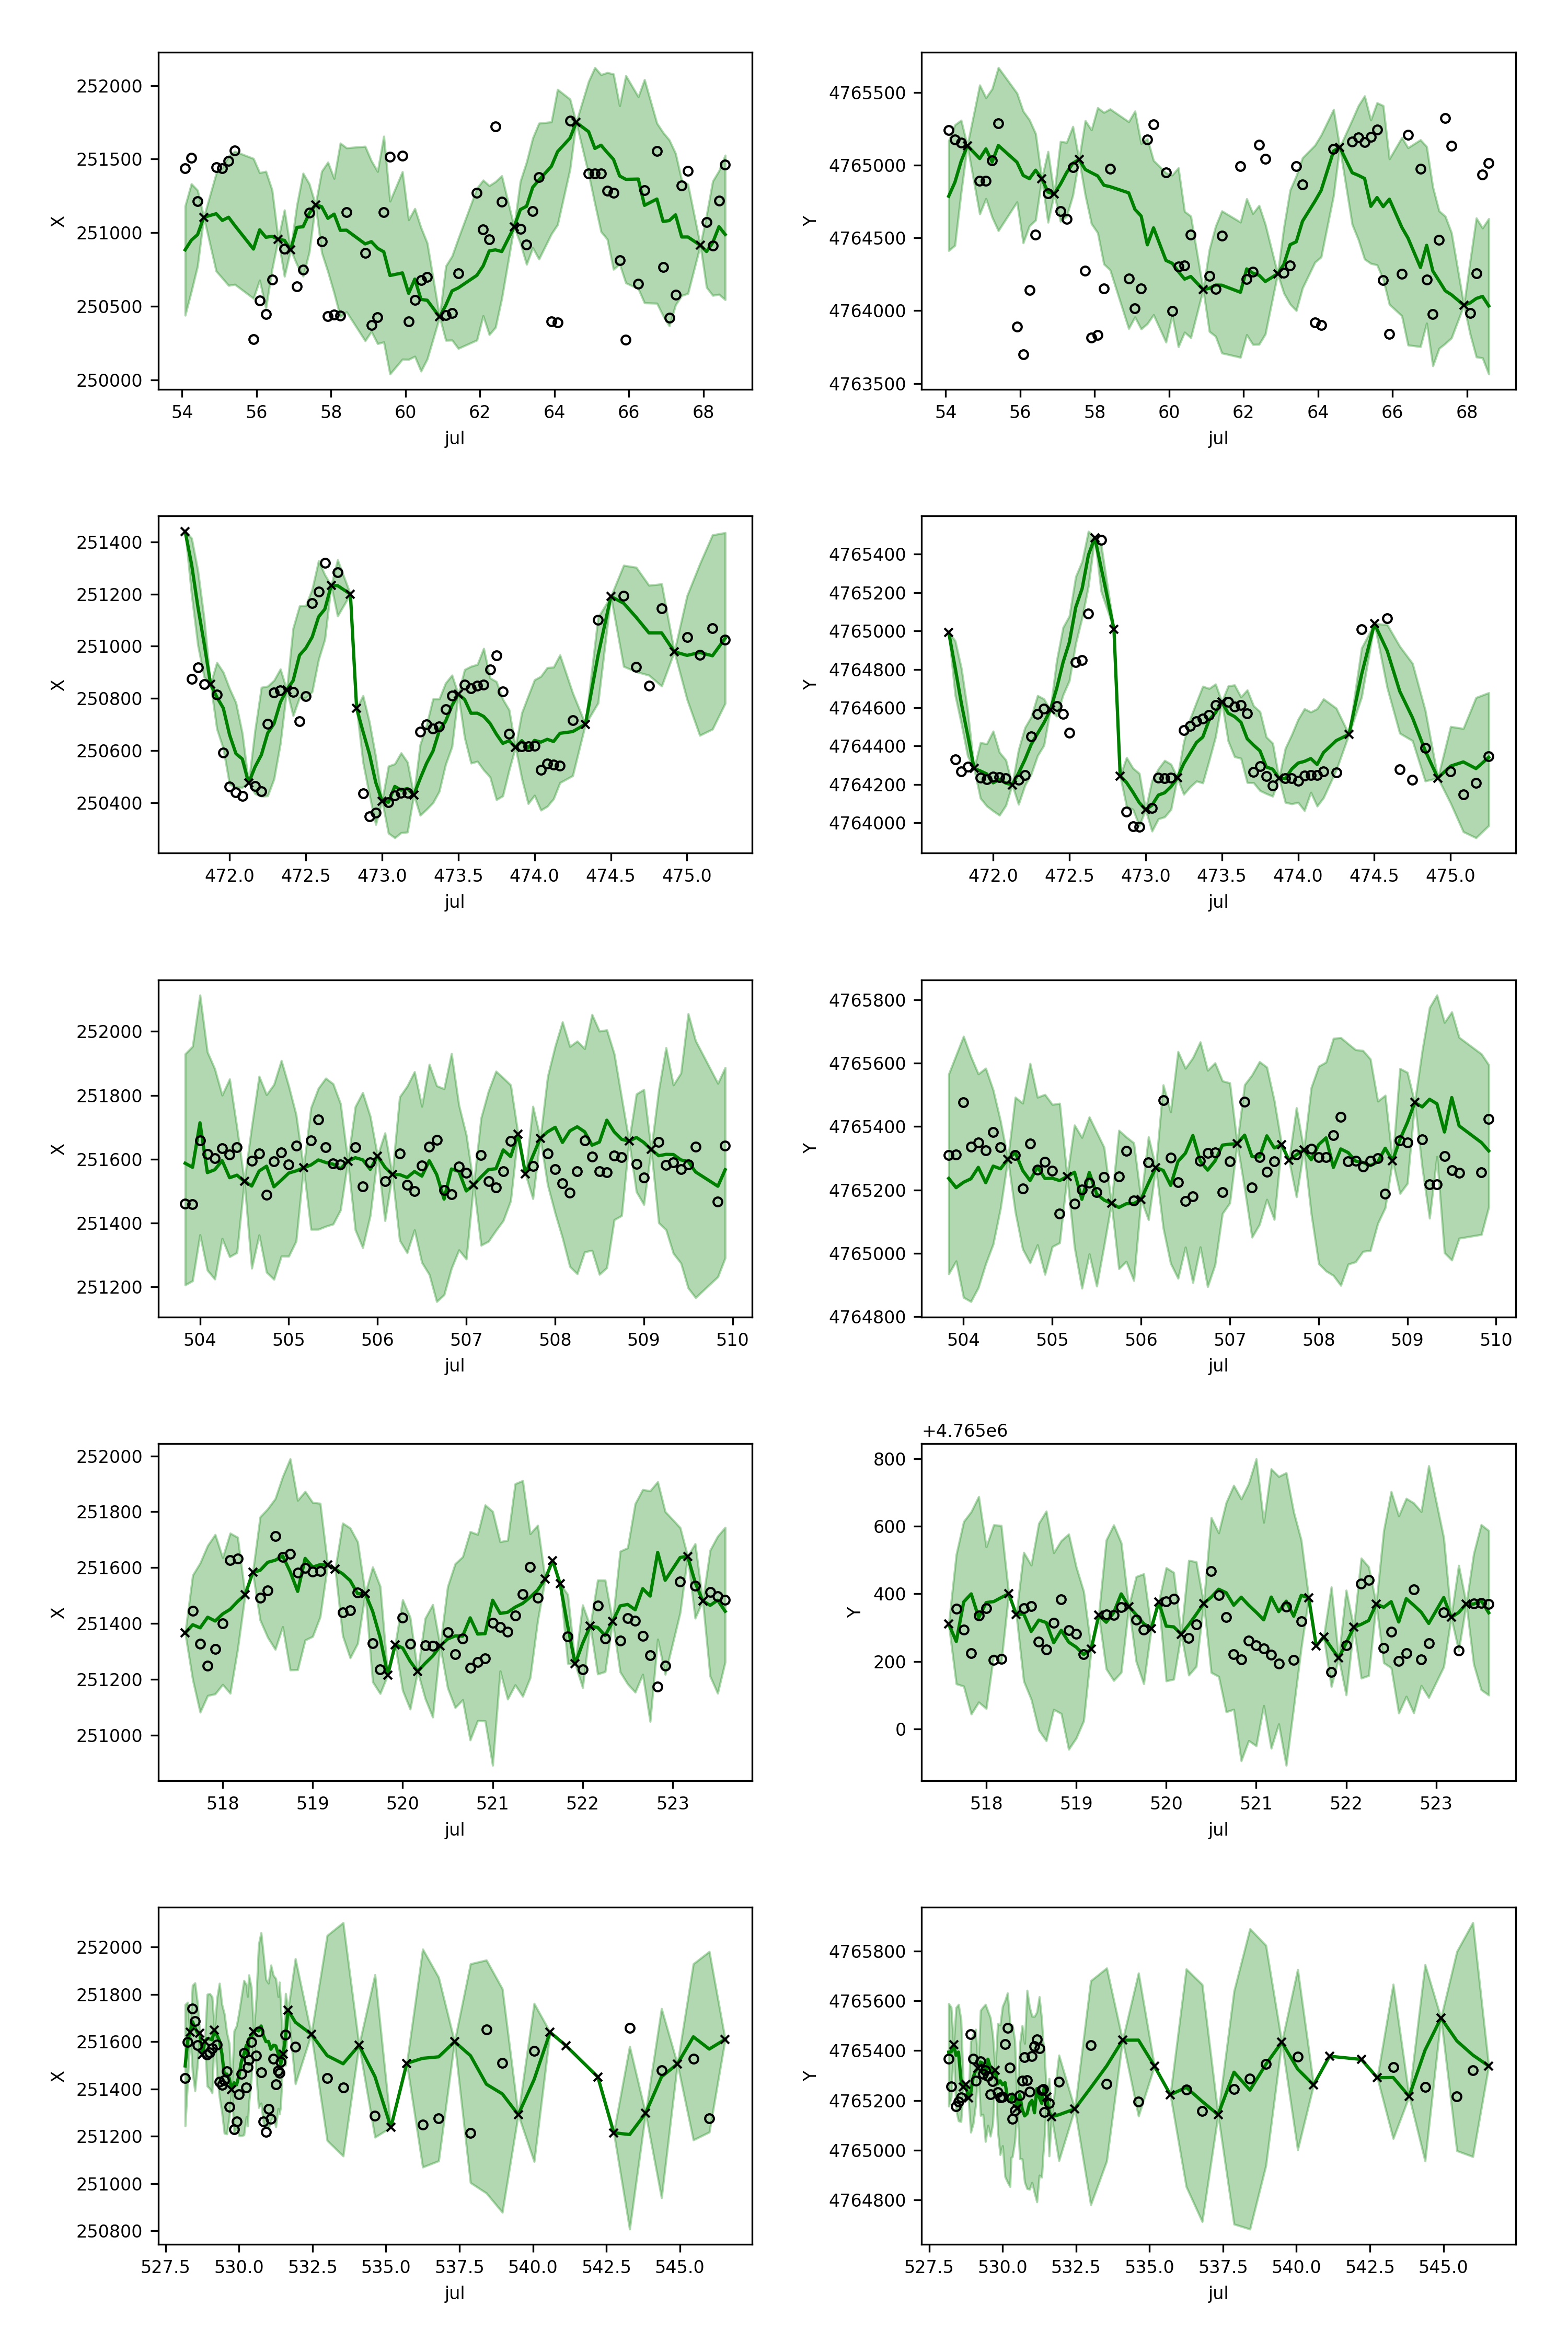
\includegraphics[width=\textwidth]{../figure/80_5094_crawl} % Adjust the scale or width as needed
  \caption{This figure illustrates the imputation results using the Continuous-Time Correlated Random Walk (CTCRW) model for a single deer's trajectory with a 80\% missing data ratio. The figure is organized into rows of subplots, with each row showing the deer's trajectory over different time windows. The left subplot in each row shows the X coordinate (longitude) against time (Julian days). The right subplot in each row shows the Y coordinate (latitude) against time. Black ``x" marks represent the observed data points, which are the actual recorded positions of the deer. Unfilled black "o" circles indicate the evaluation data points used for assessing the imputation accuracy. Solid blue lines show the imputed trajectory values generated by the CTCRW model. Shaded green areas represent the 95\% confidence interval around the imputed values.}
  \label{fig: ctcrw_80} % Label for referencing
\end{figure}

\subsection{Importance of Covariates}

We examined the impact of including additional covariates in the imputation process by testing three different scenarios: no covariates, only time-related covariates (such as month, day, and hour), and both time-related and landscape covariates. Table \ref{tab: Impact of Different Covariate Inclusion on Model Performance} presents the model performance for each scenario. Our findings indicate that, across all missing ratio scenarios, the model with the full set of covariates performs best. When the missing ratio is low (e.g., $p=20\%$), the inclusion of covariates appears less critical. This is likely because the model can rely on historical or future locations to make reasonably accurate predictions. However, as the missing ratio increases to $p=80\%$, the model that includes both time-related and landscape covariates shows a significant improvement, reducing the MAE by 12 meters. This suggests that covariates become increasingly important in aiding imputation as the missing ratio grows. This makes sense because, with sparse observations, the model struggles to accurately determine locations based solely on past and future data, and thus benefits more from additional covariate information.






\begin{table}[ht]
\centering
\begin{tabular}{|l|l|l|l|l|}
\hline
\multirow{2}{*}{\textbf{Scenario}} & \multirow{2}{*}{\textbf{Covariates}} & \multicolumn{2}{c|}{\textbf{Metrics}} \\ \cline{3-4} 
                                   &                                  & \textbf{MAE} & \textbf{CRPS} \\ \hline
\multirow{3}{*}{$p=20\%$} & time + landscape                        &123                   &    $4.4e^{-5}$               \\ \cline{2-4} 
                                   & time                        &    123              &   $4.4e^{-5}$                \\ \cline{2-4} 
                                   & none                        &     124              &      $4.5e^{-5}$             \\ \hline
\multirow{3}{*}{$p=50\%$} & time + landscape                        & 136                  &      $4.8e^{-5}$             \\ \cline{2-4} 
                                   & time                        &    138              &    $5.0e^{-5}$               \\ \cline{2-4} 
                                   & none                       &    140               &    $5.0e^{-5}$           \\ \hline
\multirow{3}{*}{$p=80\%$} & time + landscape                        & 164                  &         $6.0e^{-5}$          \\ \cline{2-4} 
                                   & time                        &   173               &   $6.5e^{-5}$               \\ \cline{2-4} 
                                   & none                        &     176             &      $6.5e^{-5}$            \\ \hline
\end{tabular}
\caption{Impact of Different Covariate Inclusion on Model Performance}
\label{tab: Impact of Different Covariate Inclusion on Model Performance}
\end{table}


\subsection{Trajectory Imputation Using CSDI}
In this section, we use the CSDI method to impute $\bm{Y}_j^{\mathrm{aug}}$, following the procedure outlined for deer trajectory imputation in the test dataset, as detailed in Section \ref{sec: model imputation}. For any $j$ in $\mathcal{D}_{\mathrm{train}} \cup \mathcal{D}_{\mathrm{test}}$, we apply Algorithm \ref{alg: trajectory imputation} to the set $\{\bm{Y}_j^{\mathrm{aug}}, \bm{Z}_j^{\mathrm{aug}}, \bm{t}_j^{\mathrm{aug}}, \bm{P}_j^{\mathrm{aug}}\}$ and obtain $B$ imputed samples, denoted by $\{\bm{Y}_j^{\mathrm{aug},b}, b=1,\ldots, B\}$. For deterministic imputation, we calculate the average of all $B$ samples, given by $\hat{\bm{Y}}_j^{\mathrm{aug}} = \frac{1}{B} \sum_{b=1}^B \bm{Y}_j^{\mathrm{aug},b}$. For probabilistic imputation, we calculate the 5\% and 95\% quantiles of the samples to estimate the "range". Visualizations of the imputation for one deer are presented in Figure \ref{fig: csdi_aug}.



\begin{figure}[h]
  \centering
  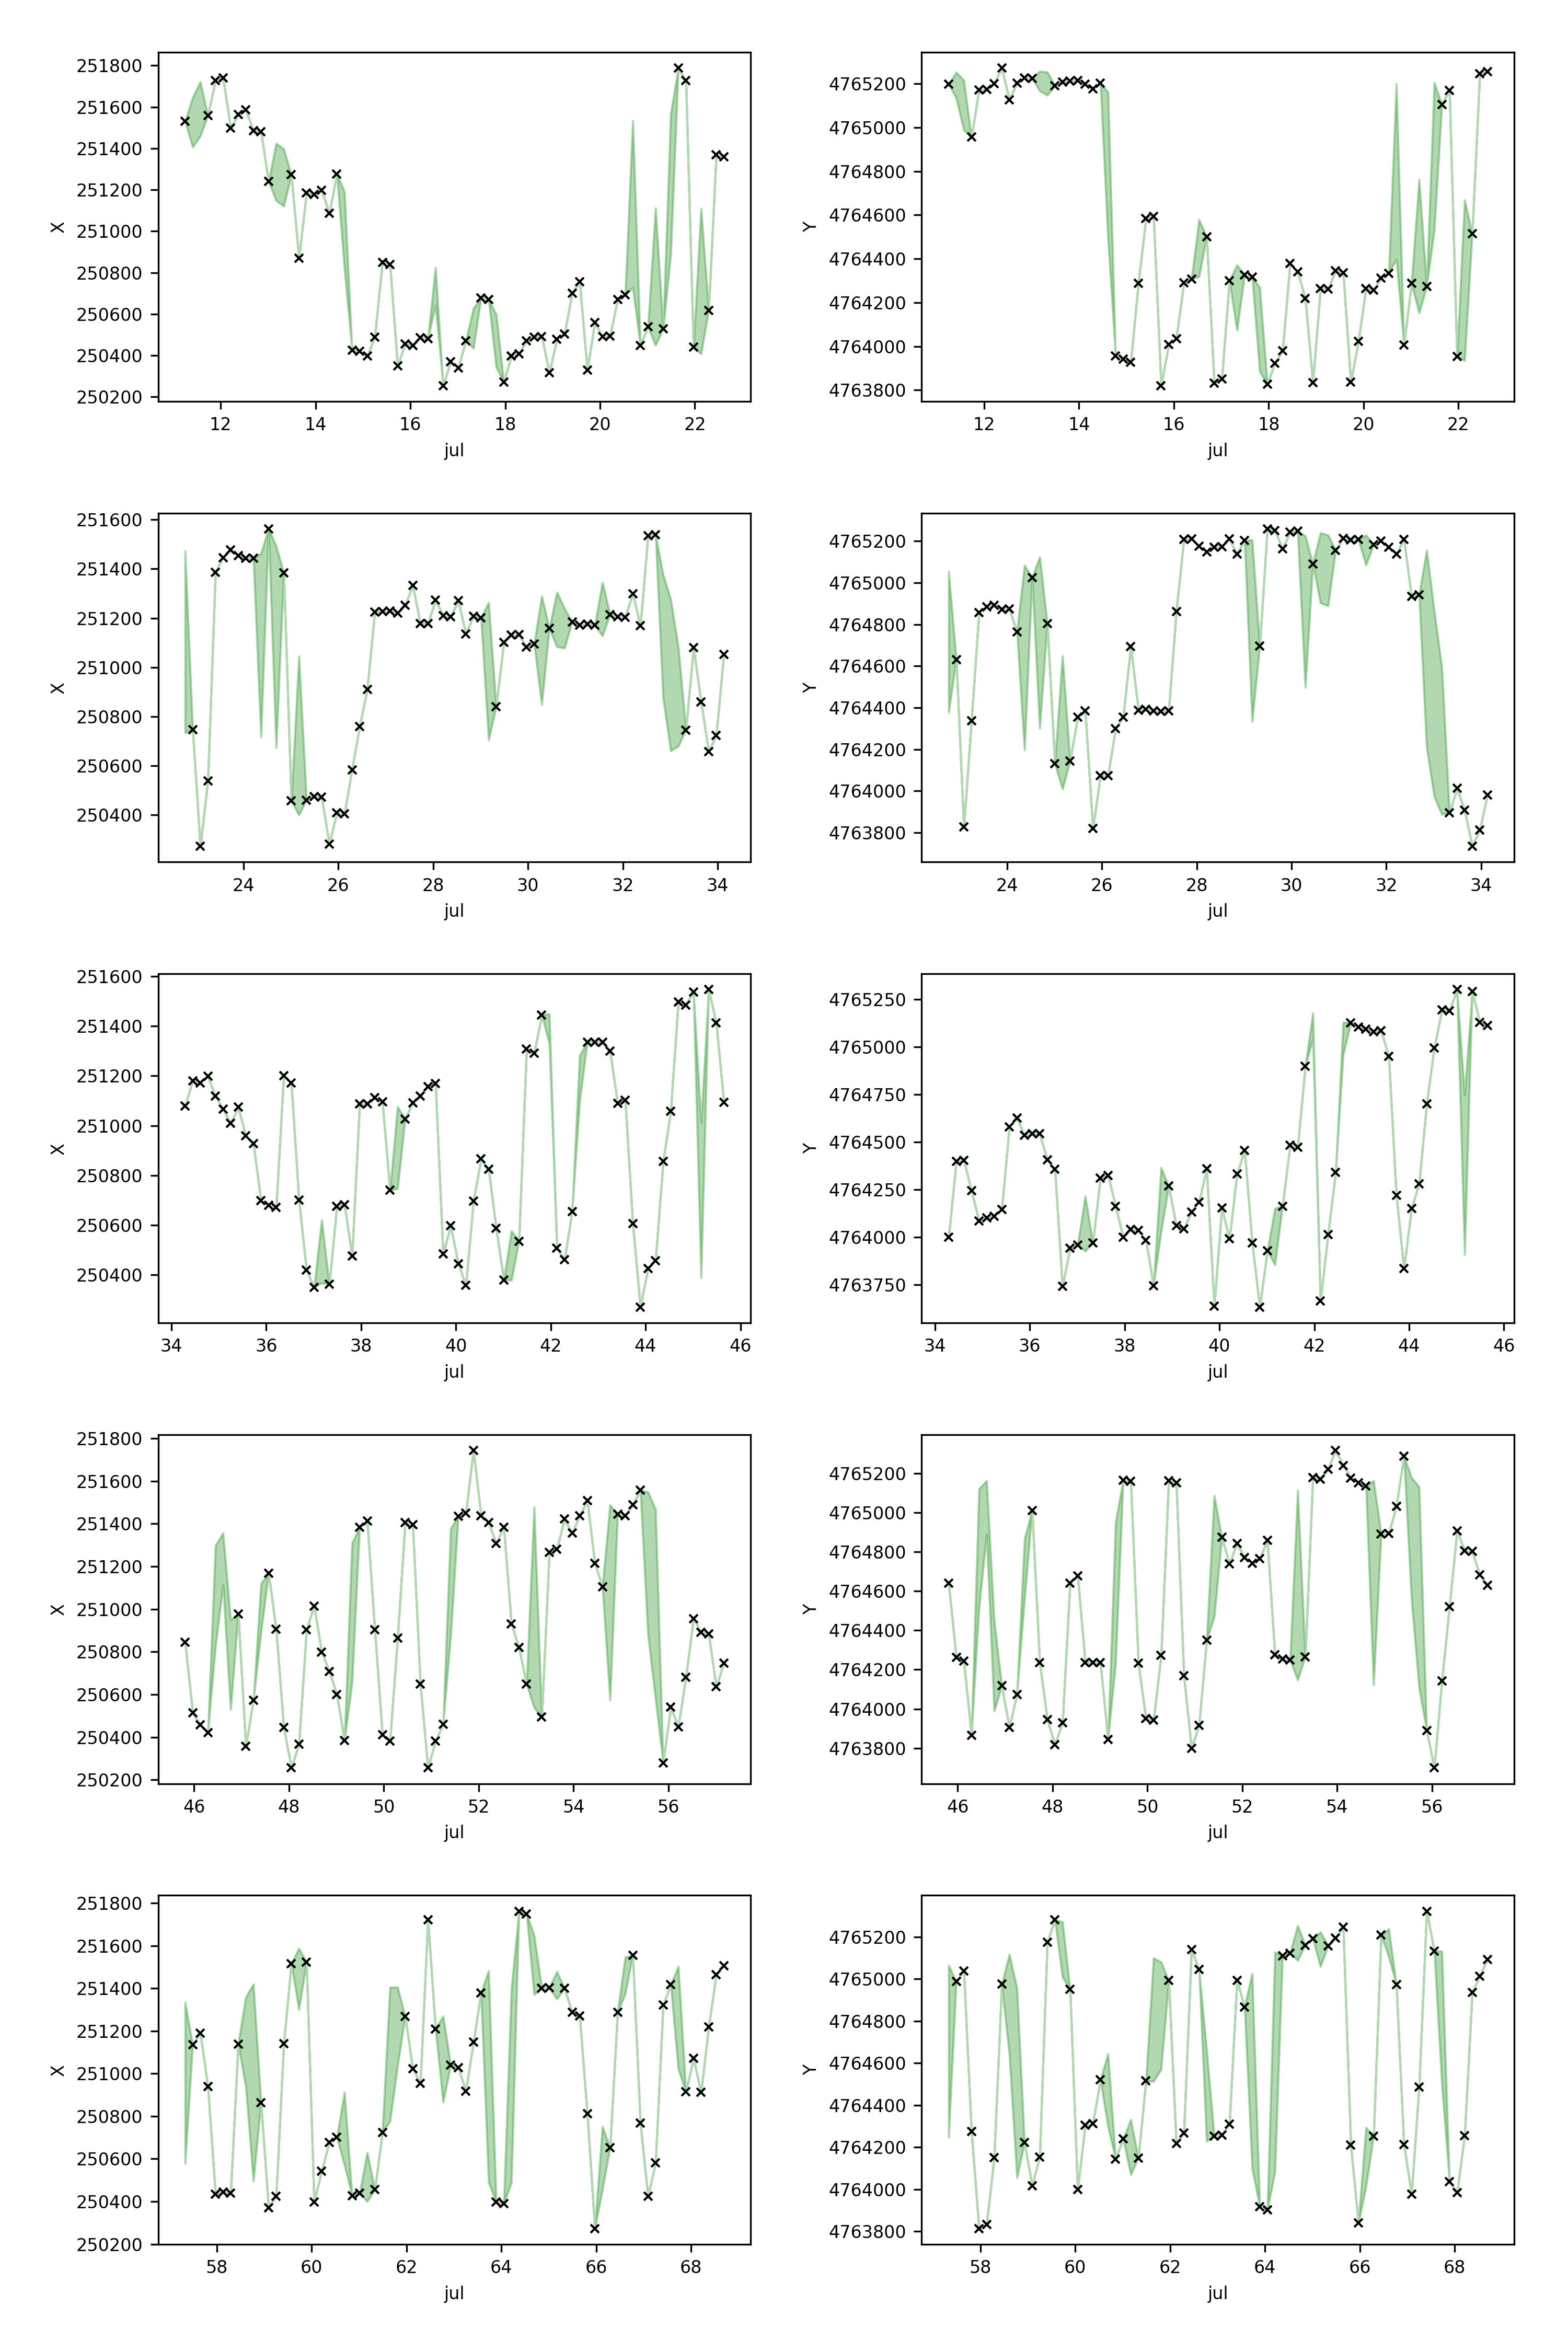
\includegraphics[width=\textwidth]{../figure/5094_4_hour_trajectory_imputation} % Adjust the scale or width as needed
  \caption{This figure illustrates the imputation results using the CSDI model for a single deer's trajectory with a 4-hour imputation interval.  The figure is organized into rows of subplots, with each row showing the deer's trajectory over different time windows. The left subplot in each row shows the X coordinate (longitude) against time (Julian days). The right subplot in each row shows the Y coordinate (latitude) against time. Black ``x" marks represent the observed data points, which are the actual recorded positions of the deer. Unfilled black "o" circles indicate the evaluation data points used for assessing the imputation accuracy. Solid blue lines show the imputed trajectory values generated by the CSDI model. Shaded green areas represent the 95\% confidence interval around the imputed values.}
  \label{fig: csdi_aug} % Label for referencing
\end{figure}



\section{Conclusion}
Our study introduces the Conditional Score-based Diffusion Model (CSDI) for animal trajectory imputation. The model can handle irregular time intervals and performs probabilistic imputation. Additionally, unlike traditional models that are applied to individual animals, this model can learn various movement patterns and conditions from a large dataset of hundreds of deer. We provide an end-to-end example from collecting animal trajectory data, training the CSDI model, comparing its performance with other methods, to finally filling the gaps in missing trajectories. In tests using Wisconsin female deer trajectory data, we showed that CSDI outperforms two traditional methods: interpolation and the continuous time random walk method in both deterministic and probabilistic imputation. Once well-trained, the model can be directly applied to the same species of animals without further training, offering a convenient tool for improved animal trajectory imputation. Since the model learns the patterns of animal movement, it can do more than imputation; for example, it can perform predictions and other analyses based on animal movement. Its potential is not limited.

\bibliographystyle{apalike}
\bibliography{refs}

\appendix

%\section{Continuous-Time Correlated Random Walk Model}\label{sec: continuous-time correlated random walk model}
%
%In the CTCRW framework, we define each animal's bivariate location data at time $t$ as $\bm{\mu}(t)=[\mu_1(t), \mu_2(t)]^{\prime}$. Define $d\bm{\mu}(t)=\bm{v}(t)dt$, where $\bm{v}(t)$ is the instantaneous rate of location change (velocity). For each coordinate axis ($c=1, 2$), we define the Ornstien-Uhlenbeck (OU) process $v_c(t)$ as follows:
%\begin{equation}\label{eq: velocity}
%    v_c(t+\Delta)=\gamma_c+e^{-\beta\Delta}[v_c(t)-\gamma_c]+\zeta_c(\Delta),
%\end{equation}
%where $\gamma_c$ is the mean velocity, $\beta$ is an autocorrelation parameter, and $\zeta_c(\Delta)$ is a zero mean normal random variable with variance $\sigma^2[1-\exp(-2\beta\Delta)]/2\beta$. The parameter $\sigma$ controls the overall variability in velocity.
%
%Using the velocity process, we obtain the continuous-time location process $\bm{\mu}(t)$ by integration as shown:
%\begin{equation}\label{eq: location}
%    \bm{\mu}(t)=\bm{\mu}(0)+\int_{0}^{t}\bm{v}(u)du.
%\end{equation}
%Equations \ref{eq: velocity} and \ref{eq: location} define the basic continuous-time correlated random walk model (CTCRW).
%
%However, the continuous path of an animal can only be observed at sampled times. Assume locations $\bm{y}_i = [y_{1i}, y_{2i}]$ are measured at times $t_1, \ldots, t_n$, and that the true locations $\bm{\mu}_i = [\mu_{1i}, \mu_{2i}]'$ of the animal at each time $t_i$ allow us to represent CTCRW within a state-space model framework. 
%
%\begin{align}\label{eq: general ssm}
%	&y_{ci}=Z_i^{\prime}\bm{\alpha}_{ci}+\epsilon_{ci}\\
%	&\bm{\alpha}_{c,i+1}=T_i\bm{\alpha}_{ci}+\bm{\eta}_{ci},
%\end{align}
%where $Z_i=[1, 0]^{\prime}$, $\bm{\alpha}_{ci}=[\mu_{ci}, v_{ci}]^{\prime}$, $\bm{\eta}_i=[\zeta_{ci}, \xi_{ci}]^{\prime}$, $H_{ci}=H(x_i)$, where $x_i$ is a known location quality covariate; and $\xi_{ci}$ are normal errors with variance 
%\begin{equation}
%	V[\xi_{ci}]=\sigma^2/\beta^2\{\Delta_i-2/\beta (1-e^{-\beta \Delta_i})+1/(2\beta)(1-e^{-2\beta\Delta_i})\}.
%\end{equation}
%
%
%\begin{equation}
%	\mathbf{T}_i=\left[\begin{array}{cc}
%1 & \left(1-e^{-\beta \Delta_i}\right) / \beta \\
%0 & e^{-\beta \Delta_i}
%\end{array}\right]
%\end{equation}
%
%\begin{equation}
%	\mathbf{Q}_{c i}=\left\{\begin{array}{cc}
%V\left[\xi_{c i}\right] & C\left[\xi_{c i}, \zeta_{c i}\right] \\
%C\left[\xi_{c i}, \zeta_{c i}\right] & V\left[\zeta_{c i}\right]
%\end{array}\right\}
%\end{equation}
%
%\begin{equation}
%	C[\zeta_{ci}, \xi_{ci}]=\sigma^2/(2\beta^2)(1-2e^{-\beta\Delta_i}+e^{-2\beta\Delta_i})
%\end{equation}
%
%
%We use the maximum likelihood method for parameter estimation and location prediction. A key advantage of the Kalman filter and smoother (KFS) is its natural handling of missing observations. To estimate the value of $\bm{\alpha}_{ci}$ at a time $t_i$ with no observed location, simply augment the dataset with $y_{ci}=\mathrm{NA}$ for that time. The KFS automatically filters and smooths the data, providing estimates for location $\hat{\bm{\alpha}}_{ci}$ and variance $\hat{V}_{ci}$. We implement this using R Statistical Software (v4.2.1) \citep{R} and the R package ``crawl" \citep{johnson2018crawl}.

%\subsection{A Continuous-Time Model}
%Denote $\bm{\mu}(t)=[\mu_1(t), \mu_2(t)]^{\prime}$ be the actual location of an animal at time $t$, with subscript 1 referring to a ``latitude" coordinate and subscript 2 referring to a ``longitude" coordinate. Then, the difference $d_{\Delta}(t)=\bm{\mu}(t+\Delta)-\bm{\mu}(t)$ describes movement of the animal over $\Delta$ time units. 
%
%If $\bm{\mu}(t)$ is a smooth and continuous path, then as $\Delta$ goes to 0, one obtains the differential equation $d\bm{\mu}(t)=\bm{v}(t)dt$, where $\bm{v}(t)$ represents the instantaneous rate of location change (velocity). For each coordinate axis, $c=1, 2$, an Ornstien-Uhlenbeck (OU) process $v_c(t)$ is defined, for each separation in time, $\Delta$, by the following autoregressive equation:
%
%\begin{equation}\label{eq: velocity}
%	v_c(t+\Delta)=\gamma_c+e^{-\beta\Delta}[v_c(t)-\gamma_c]+\zeta_c(\Delta),
%\end{equation}
%where $\gamma_c$ is the mean velocity, $\beta$ is an autocorrelation parameter, and $\zeta_c(\Delta)$ is a zero mean normal random variable with variance $\sigma^2[1-\exp(-2\beta\Delta)]/2\beta$. The parameter $\sigma$ controls the overall variability in velocity. Essentially, the equation states that velocity at time $t+\Delta$ is equal to a random variable whose variance grows with $\Delta$ plus an adjustment based on how far away the previous velocity value was from the mean. Additionally, we consider the velocity processes in each coordinate to be independent, and this assumption is realistic in the majority of cases.
%
%Using the velocity process, the continuous-time location process $\bm{\mu}(t)$ can be obtained by integration to give:
%\begin{equation}\label{eq: location}
%	\bm{\mu}(t)=\bm{\mu}(0)+\int_{0}^{t}\bm{v}(u)du.
%\end{equation}
%Equations \ref{eq: velocity} and \ref{eq: location} define the basic continuous-time correlated random walk model (CTCRW). As $\beta$ tends to $\infty$ and $\sigma/\beta$ tends to a constant, the location process becomes a standard Brownian motion (continuous-time version of a random walk). Small $\beta$ implies more directional persistence than a simple random walk. In addition, $\gamma_c=0$ usually, but could be modeled to account for drift over time.
%%
%\subsection{State-Space Model Formulation}
%The continuous path of an animal, however, can only be observed at sampled times. In addition, there are often measurement errors in the observed locations. To model animal movement, while simultaneously accounting for measurement error, we put CTCRW into a state-space model framework. 
%
%The general form of a Gaussian linear SSM for a univariate observation is given by two equations,  the observation equation and the state equation:
%
%\begin{align}\label{eq: general ssm}
%	&y_i=Z_i^{\prime}\bm{\alpha}_i+\epsilon_i\\
%	&\bm{\alpha}_{i+1}=T_i\bm{\alpha}_i+\bm{\eta}_i,
%\end{align}
%where $\bm{\alpha}_i$ is the current state vector, $y_i$ is an observation at time $i$, $T_i$ and $Z_i$ are transformation matrices, $\epsilon_i$ is a normal measurement error with variance $H_i$, and $\bm{\eta}_i$ are normal error vectors with covariance matrix $Q_i$. In the case of animal movement data, $y_i$ represents an observed location at time $t_i$ and $\bm{\alpha}_i$ is the true location and movement process of the animal at time $t_i$.
%
%Assume that locations $\bm{y}_i=[y_{1i}, y_{2i}]$ are measured at time $t_1, \ldots, t_n$, then, substituting the subscript $i$ for the argument $t_i$ and conditioning on the true location of the animal, $\bm{\mu}_i=[\mu_{1i},\mu_{2i}]^{\prime}$ at time $t_i$, we have the observation equation for the $c$th coordinate
%\begin{align}\label{eq: relation between state and observation}
%	&y_{ci}=\mu_{ci}+\epsilon_{ci}\\
%	&\epsilon_{ci}\sim N(0, H_{ci}),
%\end{align}
%where $H_{ci}$ is the measurement error variance. The error variance could depend on external location quality covariates.
%
%Next, we can form a Markovian state $\bm{\alpha}_i$, by bundling the velocity process to the location process into a single state vector. The transition equation for the velocity process is already given in \ref{eq: velocity}. The location $\mu_{c,i+1}$ can be formulated in terms of the location and velocity at time $t_i$ to obtain the following transition equation:
%\begin{equation}\label{eq: location transition function}
%	\mu_{c,i+1}=\mu_{ci}+v_{ci}(1-e^{-\beta\Delta_i}/\beta)+\xi_{ci},
%\end{equation}
%where $\Delta_i=t_{i+1}-t_i$ and $\xi_{ci}$ are normal errors with variance 
%\begin{equation}
%	V[\xi_{ci}]=\sigma^2/\beta^2\{\Delta_i-2/\beta (1-e^{-\beta \Delta_i})+1/(2\beta)(1-e^{-2\beta\Delta_i})\}.
%\end{equation}
%The covariance between $\zeta_{ci}$ and $\xi_{ci}$ is also necessary for SMM specification is given by
%\begin{equation}
%	C[\zeta_{ci}, \xi_{ci}]=\sigma^2/(2\beta^2)(1-2e^{-\beta\Delta_i}+e^{-2\beta\Delta_i})
%\end{equation}
%
%Finally, using Eqs \ref{eq: relation between state and observation}, \ref{eq: velocity} and \ref{eq: location transition function},  the CTCRW can be placed into the SSM framework for parameter estimation and prediction from observed locations with the specifications $y_{ci}=$ observed location in the $c$ coordinate at time $t_i$; $Z_i=[1, 0]^{\prime}$, $\bm{\alpha}_{ci}=[\mu_{ci}, v_{ci}]^{\prime}$, $\bm{\eta}_i=[\zeta_{ci}, \xi_{ci}]^{\prime}$, $H_{ci}=H(x_i)$, where $x_i$ is a known location quality covariate; and 
%
%\begin{equation}
%	\mathbf{T}_i=\left[\begin{array}{cc}
%1 & \left(1-e^{-\beta \Delta_i}\right) / \beta \\
%0 & e^{-\beta \Delta_i}
%\end{array}\right]
%\end{equation}
%
%\begin{equation}
%	\mathbf{Q}_{c i}=\left\{\begin{array}{cc}
%V\left[\xi_{c i}\right] & C\left[\xi_{c i}, \zeta_{c i}\right] \\
%C\left[\xi_{c i}, \zeta_{c i}\right] & V\left[\zeta_{c i}\right]
%\end{array}\right\}
%\end{equation}
%
%
%\subsection{Statistical Inference}
%We use the maximum likelihood method of parameter estimation and location prediction. When using SSMs, the Kalman filter (KF) is a fast and efficient computing method for finding maximum likelihood estimates of movement parameters $\hat{\theta}=[\hat{\beta}_1, \hat{\beta}_2, \hat{\sigma}_1, \hat{\sigma}_2]^{\prime}$. In addition, optimum predictions and prediction intervals of unobserved locations, $\hat{\bm{\mu}}(t)$, can be obtained as a by-product.
%
%\subsection{Kalman Filter Equations}
%
%The Kalman filter recursions are an invaluable tool when modeling time series with an SSM. Because we are considering independent processes of movement in each coordinate direction, we formulate the filtering and estimation in terms of two one-dimensional series of observations. The Kalman filter recursions for the CTCRW model are given by
%\begin{align}
%	&v_{ci}=y_{ci}-Z_i^{\prime}\bm{\alpha}_{ci}\\
%	&F_{ci}=Z_i^{\prime}P_{ci}Z_i+H_{ci}\\
%	&K_{ci} = T_i P_{ci}Z_i/F_{ci}\\
%	&L_{ci}=T_i-K_{ci}Z_i^{\prime}\\
%	&\bm{\alpha}_{c,i+1}=T_i\bm{\alpha}_{ci}+K_{ci}v_{ci}\\
%	&P_{c,i+1}=T_iP_P{ci}L_{ci}^{\prime}+Q_{ci},
%\end{align}
%for $i=1,\ldots, n$ and $c=1,2$. We set $\bm{\alpha}_{c1}=[y_{c1}, 0]^{\prime}$ and a ``large" covariance matrix for $P_{c1}$.
%
%Due to the fact $\epsilon_i$ and $\bm{\eta}_i$ are Gaussian, the log-likelihood is 
%\begin{equation}
%	L(\bm{\theta})=-n\log 2\pi - 1/2\sum_{c=1}^2\sum_{i=1}^{n}(\log F_{ci} + v_{ci}^2/F_{ci}),
%\end{equation}
%where $\bm{\theta}$ is a vector of all model parameters. The log-likelihood can be optimized to provide parameter values for state estimation. 
%
%Estimation of the state processes involves running the Kalman filter forward and then running a set of smoothing recursions backward through the series \citep{durbin2012time} to obtain the state estimates $\hat{\bm{\alpha}}_{ci}$ and variance estimates $\hat{V}_{ci}$. The smoothing recursions for each coordinate are given by
%
%\begin{align}
%	&\bm{r}_{c,i-1}=Z_iv_{ci}/F_{ci}+L_{ci}^{\prime}\bm{r}_{ci}\\
%	&N_{c,i-1}=Z_iZ_i^{\prime}/F_{ci}+L_{ci}^{\prime}N_{ci}L_{ci}\\
%	&\hat{\bm{\alpha}}_{ci}=\bm{\alpha}_{ci}+P_{ci}\bm{r}_{c,i-1}\\
%	&\hat{V}_{ci}=P_{ci}-P_{ci}N_{c,i-1}P_{ci}
%\end{align}
%for $i=n,\ldots, 1$ and $c=1,2$, where $\bm{r}_{cn}=\bm{0}$, $N_{cn}=\bm{0}$. The combined filter and smoothing recursions are known as the Kalman filter and smoother.
%
%One benefit of using the Kalman filter and smoother (KFS) is that it handles missing observations naturally. If one would like an estimated value of $\bm{\alpha}_{ci}$ for at a time $t_i$ when no location was observed, all we need to do is to augment the dataset with missing $y_{ci}=\mathrm{NA}$ at that time. The KFS automatically filters and smooths to provide location and variance estimates $\hat{\bm{\alpha}}_{ci}$ and $\hat{V}_{ci}$. This is accomplished by setting $v_{ci}=0$, $K_{ci}=0$ and $N_{c,i-1}=T_iN_{ci}T_i$ for observation time $t_i$.
%



\section{Details of Denoising Diffusion Probabilistic Models}\label{sec: DDPM details}
This section details the denoising diffusion probabilistic models discussed in Section \ref{sec: ddpm}.
Introduced in Equations \ref{eq: forward diffusion} and \ref{eq: reverse diffusion}, diffusion models are latent variable models comprising two main processes: the forward process, which gradually adds noise to the data, and the reverse process, which removes this noise to either reconstruct the original data or generate new data.
The objective is to adjust the parameters $\theta$ to maximize the likelihood's variational lower bound (ELBO), expressed as $p_{\theta}(\mathbf{X}_{0:T})$:
\begin{equation}
    \mathbb{E}_{q(\mathbf{X}_0)}\left\{\log p_{\theta}(\mathbf{X}_0)\right\} \geq \mathbb{E}_{q(\mathbf{X}_0,\mathbf{X}_1,\ldots,\mathbf{X}_T)}\left\{\log p_{\theta}(\mathbf{X}_{0:T})-\log q(\mathbf{X}_{1:T}|\mathbf{X}_0)\right\} := \text{ELBO}.
\end{equation}

\citet{ho2020denoising} developed denoising diffusion probabilistic models (DDPM) and introduced a parametrization that simplifies the Evidence Lower Bound (ELBO). Using this parametrization, they showed that the ELBO satisfies:
\begin{equation}
    -\text{ELBO} = c + \sum_{t=1}^T \kappa_t \mathbb{E}_{\mathbf{X}_0 \sim q(\mathbf{X}_0), \boldsymbol{\epsilon} \sim \mathcal{N}(\mathbf{0}, \bm{\mathrm{I}})}\left\|\boldsymbol{\epsilon} - \boldsymbol{\epsilon}_\theta\left(\sqrt{\alpha_t} \mathbf{X}_0 + (1-\alpha_t) \boldsymbol{\epsilon}, t\right)\right\|_2^2,
\end{equation}
Here, $c$ is a constant, and $\{\kappa_{1:T}\}$ are positive coefficients that depend on $\alpha_{1:T}$ and $\beta_{1:T}$. This formulation implies that training the diffusion process requires minimizing the ELBO.

Furthermore, \citet{ho2020denoising} found that minimizing an unweighted version of the ELBO yields high-quality samples:
\begin{equation}
    \min_{\theta} \mathcal{L}(\theta) := \min_{\theta} \mathbb{E}_{\mathbf{X}_0 \sim q(\mathbf{X}_0), \boldsymbol{\epsilon} \sim \mathcal{N}(\mathbf{0}, \bm{\mathrm{I}}), t}\left\|\boldsymbol{\epsilon} - \boldsymbol{\epsilon}_\theta\left(\sqrt{\alpha_t} \mathbf{X}_0 + (1-\alpha_t) \boldsymbol{\epsilon}, t\right)\right\|_2^2,
\end{equation}
Here, the function $\boldsymbol{\epsilon}_{\theta}$ is trained to estimate the noise $\boldsymbol{\epsilon}$ in the noisy input. Once trained, the model samples $\mathbf{X}_0$ using the reverse diffusion equation \ref{eq: reverse diffusion}.

%In this section, we provide the details of denoising diffusion probabilistic models in Section \ref{sec: ddpm}.
%Diffusion models \ref{eq: forward diffusion} are a type of latent variable model consisting of two main processes: a forward process, which gradually adds noise to data, and a reverse process, which aims to remove this noise to reconstruct the original data or generate new data. These processes are defined in Eq. \ref{eq: forward diffusion} and Eq. \ref{eq: reverse diffusion}, respectively. 
%
%The learning objective is to adjust the parameters $\theta$ to maximize variational lower bound (ELBO) of likelihood $p_{\theta}(\bm{X}_{0:T})$:
%\begin{equation}\label{eq: ELBO}
%	E_{q(\bm{X}_0)}\{\log p_{\theta}(\bm{X}_0)\}\geq E_{q(\bm{X}_0,\bm{X}_1,\ldots,\bm{X}_T)}\{\log p_{\theta}(\bm{X}_{0:T})-\log q(\bm{X}_{1:T}|\bm{X}_0)\}:=\mathrm{ELBO}.
%\end{equation}
%To analyze this ELBO, \citet{ho2020denoising} proposed denoising diffusion probabilistic models (DDPM), which considered the parametrization given by \ref{eq: DDPM parametrization}. Under the parametrization, \citet{ho2020denoising} showed ELBO satisfies the following equation:
%\begin{equation}
%	-\mathrm{ELBO}=c+\sum_{t=1}^T \kappa_t E_{\mathbf{x}_0 \sim q\left(\mathbf{x}_0\right), \boldsymbol{\epsilon} \sim N(\mathbf{0}, I)}\left\|\boldsymbol{\epsilon}-\boldsymbol{\epsilon}_\theta\left(\sqrt{\alpha_t} \mathbf{x}_0+\left(1-\alpha_t\right) \boldsymbol{\epsilon}, t\right)\right\|_2^2
%\end{equation}
%where $c$ is a constant and $\{\kappa_{1:T}\}$ are positive coefficients depending on $\alpha_{1:T}$ and $\beta_{1:T}$. The diffusion process can be trained by minimizing \ref{eq: ELBO}. In addition, \citet{ho2020denoising} found that minimizing the following unweighted version of ELBO leads to good sample quality:
% 
%\begin{equation}
%	\min _\theta L(\theta):=\min _\theta E_{\mathbf{x}_0 \sim q\left(\mathbf{x}_0\right), \boldsymbol{\epsilon} \sim N(\mathbf{0}, I), t}\left\|\boldsymbol{\epsilon}-\boldsymbol{\epsilon}_\theta\left(\sqrt{\alpha_t} \mathbf{x}_0+\left(1-\alpha_t\right) \boldsymbol{\epsilon}, t\right)\right\|_2^2
%\end{equation}
%The function $\bm{\epsilon}_{\theta}$ estimates noise $\bm{\epsilon}$ in the noisy input. Once trained, we sample $\bm{x}_0$ from Eq. \ref{eq: reverse diffusion}.

%\section{Algorithms of CSDI}
%\subsection{Target Choice Strategies for Self-Supervised Training}
%We use the following algorithm to select imputation targets. 
%\begin{algorithm}
%\caption{Target choice with the random strategy}
%
%1. \textbf{Input:} a training sample $x_0$\\
%2. \textbf{Output:} conditional information $\bm{x}_{0}^{co}$, imputation targets $\bm{x}_{0}^{ta}$\\
%3. Draw target ratio $r \sim \text{Uniform}(0, 100)$
%Randomly choose $r\%$ of the observed values of $\bm{x}_0$ and denote the chosen observations as $\bm{x}_{0}^{ta}$, and denote the remaining observations as $\bm{x}_{0}^{co}$.
%
%\end{algorithm}


%\subsection{Algorithm for Training and Sampling of CSDI}
%We provide the training procedure of CSDI in Algorithm \ref{alg: training} and imputation (sampling) procedure with CDSI in Algorithm \ref{alg: imputation}
%
%\begin{algorithm}\label{alg: training}
%\caption{Training of CSDI}
%1. \textbf{Input:} distribution of training data $q(\bm{x}_0)$, the number of iterations $N_{iter}$, the sequence of noise levels $\{\alpha_t\}$.\\
%2. \textbf{Output:} Trained denoising function $\bm{\epsilon}_{\theta}$.\\
%3. \textbf{for} i=1 \textbf{to} $N_{iter}$ \textbf{do}\\
%4. \quad $t\sim$ Uniform$(\{1,\ldots, T\})$, $\bm{x}_0\sim q(\bm{x}_0)$.\\
%5. \quad Separate observed values of $\bm{x}_0$ into conditional information $\bm{x}_0^{co}$ and imputation targets $\bm{x}_0^{ta}$ by random strategy.\\
%6. \quad $\bm{\epsilon}\sim N(\bm{0}, I)$ where the dimension of $\bm{\epsilon}$ corresponds to $\bm{x}_0^{ta}$.\\
%7. \quad Calculate noisy targets $\bm{x}_t^{ta}=\sqrt{\alpha}_t \bm{x}_0^{ta} + (1-\alpha_t)\bm{\epsilon}$.\\
%8. \quad Take gradient step on $\nabla_\theta\left\|\left(\boldsymbol{\epsilon}-\boldsymbol{\epsilon}_\theta\left(\mathbf{x}_t^{\mathrm{ta}}, t \mid \mathbf{x}_0^{\mathrm{co}}\right)\right)\right\|_2^2$.
%\end{algorithm}
%
%\begin{algorithm}\label{alg: imputation}
%\caption{Imputation (Sampling) with CSDI}
%1. \textbf{Input:} a data sample $\bm{x}_0$, trained denoising function $\bm{\epsilon}_{\theta}$.\\
%2. \textbf{Output:} Imputed missing values $\bm{x}_0^{ta}$.\\
%3. Denote observed values of $\bm{x}_0$ as $\bm{x}_0^{co}$.\\
%4. $\bm{x}_T^{ta}\sim N(\bm{0}, I)$ where the dimension of $\bm{x}_T^{ta}$ corresponds to the missing indices of $\bm{x}_0$.\\
%5. \textbf{for} $t=T$ \textbf{to} 1 \textbf{do}\\
%6. \quad Sample $\bm{x}_{t-1}^{ta}$ using \ref{eq: conditional reverse process} and \ref{eq: conditional DDPM parametrization}.
%\end{algorithm}

%\section{Details of Architectures and Experiment Setting}
%\subsection{Details of Implementation of CSDI}
%We describe the details of architectures and hyperparameters for the conditional diffusion model described in Section \ref{sec: csdi}. First, we provide the whole architecture of CSDI in Figure (). Since the architecture is based on DiffWave \citep{kong2020diffwave}, we mainly explain the difference from DiffWave. 
%
%On the top of the figure, the models take $\bm{x}_0^{co}$ and $\bm{x}_t^{ta}$ as inputs since $\bm{\epsilon}_{\theta}$ is the conditional denoising function. For the diffusion step $t$, we use the following 128-dimension embedding following previous works \citep{vaswani2017attention}.
%\begin{equation}
%	t_{embedding}(t)=\{\sin(10^{0\cdot 4/63}t),\ldots, \sin(10^{63\cdot 4/63}t), \cos(10^{0\cdot 4/63}t),\ldots,\cos(10^{63\cdot 4/63}t)\}.
%\end{equation}
%Similarly, we use time embeddings of $\bm{s}=\{s_{1:L}\}$ as a side information. We also use a 128-dimension temporal embedding following previous works \citep{vaswani2017attention}.
%\begin{equation}
%	s_{embedding}(s_l)=\{\sin(s_l/\tau^{0/64}),\ldots, \sin(s_l/\tau^{63/64}), \cos(s_l/\tau^{0/64}),\ldots,\cos(s_l/\tau^{63/64})\},
%\end{equation}
%where $\tau=10000$. On the top right of the figure, we expand each side information and concatenate all the side information. On the bottom right of the figure, we multiply the output by a mask $1-\bm{m}^{co}$ to mask the indices of the conditional observations of the output. 
%
%As for Transformer layers, we used a 1-layer TransformerEncoder implemented in PyTorch \citep{paszke2019pytorch}, which is composed of a multi-head attention layer, fully connected layers, and layer normalization.
%
%As for hyperparameters, we set the batch size to 16 and the number of epochs to 500. We used the Adam optimizer with a learning rate of 0.001 (cosine scheduler with restarts). As for the model, we set the number of residual layers as 4, residual channels as 64, and attention heads as 8. The number of the parameter in the model is about 423000.
%
%We also provide hyperparameters for the diffusion model as follows. We set the number of the diffusion step $T=50$, the minimum noise level $\beta_1=0.0001$, and the maximum noise level $\beta_T=0.5$. Since recent studies \citet{song2020denoising} reported that gentle decay of $\alpha_t$ could improve the sample quality, we adopted the following quadratic schedule for other noise levels:
%\begin{equation}
%	\beta_t=\big(\frac{T-t}{T-1}\sqrt{\beta_1}+\frac{t-1}{T-1}\sqrt{\beta_T}\big)^2
%\end{equation}


%\section{RandomForest}\label{sec: randomforest}
%In this section, we briefly describe the steps of training the RandomForest model based on $\{\bm{Y}_j,\bm{Z}_j,\bm{t}_j\}$, where $j\in \mathcal{D}_{\mathrm{train}}$. 
%We train the RandomForest model on all deer $j\in \mathcal{D}_{\mathrm{train}}$. The training target value is bivariate location at time $t$, the features used for predictions are the historical bivariate locations and future locations in a certain window, plus the side informaiton including covariates at all observed locations. Once the training is over, we are given an optimized random forest model, which an be used for interpolating missing observation points. To construct and train the model, we used scikit-learn \cite{scikitlearnRandomForest}, a python machine learning package.

\end{document}